\documentclass[fleqn,10pt]{wlscirep}
%DIF LATEXDIFF DIFFERENCE FILE
%DIF DEL /Users/carmen/Library/CloudStorage/OneDrive-TheUniversityofLiverpool/research/paper-submissions/2025/latin-mobility-covid/nature-communications/original/main.tex   Thu Dec 18 17:13:03 2025
%DIF ADD /Users/carmen/Library/CloudStorage/OneDrive-TheUniversityofLiverpool/research/paper-submissions/2025/latin-mobility-covid/nature-communications/r1/main-r1.tex      Thu Dec 18 21:03:00 2025
\usepackage[utf8]{inputenc}
\usepackage{units}
\usepackage{makecell}
\usepackage{float}
\usepackage[T1]{fontenc}
\title{Sustained changes to urban mobility after COVID-19 amplified socio-economic inequalities in Latin America}



\author[1,2,*,\textsuperscript{\textdagger}]{Carmen Cabrera}
%DIF 12-13c12-13
%DIF < \author[3]{Miguel González-Leonardo}
%DIF < \author[1]{Andrea Nasuto}
%DIF -------
\author[1]{Miguel González-Leonardo} %DIF > 
\author[1,3]{Andrea Nasuto} %DIF > 
%DIF -------
\author[2]{Ruth Neville}
\author[1,\textsuperscript{\textdagger}]{Francisco Rowe}
\affil[1]{Geographic Data Science Lab, Department of Geography and Planning, University of Liverpool, Liverpool, UK}
\affil[2]{Centre for Advanced Spatial Analysis, University College London, London, UK}
%DIF 18c18
%DIF < \affil[3]{Centre for Demographic Urban and Environmental Studies, El Colegio de México, México City, México}
%DIF -------
\affil[3]{Institute for Quantitative Social Science, Harvard University, Cambridge, US} %DIF > 
%DIF -------


%DIF 21d21
%DIF < 
%DIF -------
\affil[*]{Corresponding author: c.cabrera@liverpool.ac.uk}

\affil[ \textsuperscript{\textdagger}]{These authors have contributed equally to this study.}

%\keywords{Keyword1, Keyword2, Keyword3}


\begin{abstract}
%DIF 30c29
%DIF < Urban mobility is central to economic activity, social inclusion and access to services. COVID-19 caused disruptions to mobility globally, yet its long-term impacts in less developed countries remain poorly understood. Using an unprecedentedly large dataset of $>$170 million mobile phone records from Meta-Facebook users in Argentina, Chile, and Colombia (March 2020–May 2022), we find sustained changes in mobility across socioeconomic and rural–urban gradients. We reveal that mobility recorded the sharpest declines and remained below pre-pandemic levels in most high-density and low socio-economic deprivation areas, while low-density and more deprived communities returned to baseline. These differences reflect the scale of the initial mobility shock, rather than subsequent recovery rates. Our findings reveal how a global shock can entrench disparities in human mobility, with implications for economic resilience, social inclusion and urban planning in unequal nations. Our study underscores the need for proactive policies to prevent long‑lasting inequalities in mobility.
%DIF -------
Urban mobility is central to economic activity, social inclusion and access to services. COVID-19 caused disruptions to mobility globally, yet its long-term impacts in less developed countries remain poorly understood. Using an unprecedentedly large dataset of $>$170 million mobile phone records from Meta-Facebook users in Argentina, Chile and Colombia (April 2020–May 2022), we find sustained changes in mobility across socioeconomic and rural–urban gradients. We reveal that mobility recorded the sharpest declines and remained below pre-pandemic levels in most high-density and most affluent areas, while low-density and more deprived communities returned to baseline. These differences reflect the scale of the initial mobility shock, rather than subsequent recovery rates. Our findings reveal how a global shock can entrench disparities in human mobility, with implications for economic resilience, social inclusion and urban planning in unequal nations. Our study underscores the need for proactive policies to prevent long‑lasting inequalities in mobility. %DIF > 
%DIF -------

%The COVID-19 pandemic caused unprecedented disruptions to urban mobility patterns. Existing work has overwhelmingly focused on the immediate impacts of COVID-19 on human mobility during 2020, particularly in more developed countries. It showed that COVID-19 restrictions led to unequal effects: greater reductions in mobility in less deprived and high-density areas than in more deprived and less dense communities. However, little is known about the long-term persistence of these unequal impacts beyond 2020, and in less developed countries where socioeconomic disparities are more acute. Using over 100 million anonymised daily records of mobile phone data from Meta-Facebook users from March 2020 to May 2022, we aim to determine the long-term geographic and socioeconomic impact of COVID-19 on mobility patterns in Latin American countries (Argentina, Chile and Colombia). Our findings reveal sustained differences in mobility after the immediate effects of COVID-19 in 2020 extending beyond early 2022. Less deprived and high-density areas continued to display lower mobility levels than more deprived and less dense communities. We also show that the magnitude of the initial mobility reduction largely determined the extent of differences in mobility levels across socioeconomic groups over time. We find a sustained reduction in net mobility flows in core and dense urban areas, suggesting that cities lost attraction power as daily centres of gravity. Our findings suggest that the COVID-19 pandemic has contributed to amplified pre-existing socioeconomic inequalities. Targeted interventions to close the recovery gap need to be directed to support mobility in hard-hit urban centres (e.g. reconfiguring urban public transit), rural areas (reconnecting isolated communities) and assisting more deprived communities (mitigating travel costs). Overall, our research contributes evidence to building more resilient mobility systems that allow returning to daily life more efficiently and equitably after major disaster shocks.

\end{abstract}
%DIF PREAMBLE EXTENSION ADDED BY LATEXDIFF
%DIF UNDERLINE PREAMBLE %DIF PREAMBLE
\RequirePackage[normalem]{ulem} %DIF PREAMBLE
\RequirePackage{color}\definecolor{RED}{rgb}{1,0,0}\definecolor{BLUE}{rgb}{0,0,1} %DIF PREAMBLE
\providecommand{\DIFadd}[1]{{\protect\color{blue}\uwave{#1}}} %DIF PREAMBLE
\providecommand{\DIFdel}[1]{{\protect\color{red}\sout{#1}}}                      %DIF PREAMBLE
%DIF SAFE PREAMBLE %DIF PREAMBLE
\providecommand{\DIFaddbegin}{} %DIF PREAMBLE
\providecommand{\DIFaddend}{} %DIF PREAMBLE
\providecommand{\DIFdelbegin}{} %DIF PREAMBLE
\providecommand{\DIFdelend}{} %DIF PREAMBLE
\providecommand{\DIFmodbegin}{} %DIF PREAMBLE
\providecommand{\DIFmodend}{} %DIF PREAMBLE
%DIF FLOATSAFE PREAMBLE %DIF PREAMBLE
\providecommand{\DIFaddFL}[1]{\DIFadd{#1}} %DIF PREAMBLE
\providecommand{\DIFdelFL}[1]{\DIFdel{#1}} %DIF PREAMBLE
\providecommand{\DIFaddbeginFL}{} %DIF PREAMBLE
\providecommand{\DIFaddendFL}{} %DIF PREAMBLE
\providecommand{\DIFdelbeginFL}{} %DIF PREAMBLE
\providecommand{\DIFdelendFL}{} %DIF PREAMBLE
%DIF COLORLISTINGS PREAMBLE %DIF PREAMBLE
\RequirePackage{listings} %DIF PREAMBLE
\RequirePackage{color} %DIF PREAMBLE
\lstdefinelanguage{DIFcode}{ %DIF PREAMBLE
%DIF DIFCODE_UNDERLINE %DIF PREAMBLE
  moredelim=[il][\color{red}\sout]{\%DIF\ <\ }, %DIF PREAMBLE
  moredelim=[il][\color{blue}\uwave]{\%DIF\ >\ } %DIF PREAMBLE
} %DIF PREAMBLE
\lstdefinestyle{DIFverbatimstyle}{ %DIF PREAMBLE
	language=DIFcode, %DIF PREAMBLE
	basicstyle=\ttfamily, %DIF PREAMBLE
	columns=fullflexible, %DIF PREAMBLE
	keepspaces=true %DIF PREAMBLE
} %DIF PREAMBLE
\lstnewenvironment{DIFverbatim}{\lstset{style=DIFverbatimstyle}}{} %DIF PREAMBLE
\lstnewenvironment{DIFverbatim*}{\lstset{style=DIFverbatimstyle,showspaces=true}}{} %DIF PREAMBLE
%DIF END PREAMBLE EXTENSION ADDED BY LATEXDIFF

\begin{document}

\flushbottom
\maketitle
% * <john.hammersley@gmail.com> 2015-02-09T12:07:31.197Z:
%
%  Click the title above to edit the author information and abstract
%
\thispagestyle{empty}

Cities were epicentres of the COVID-19 pandemic. By November 2020, approximately 95\% of all the reported infections and fatalities had concentrated in a few large cities \cite{Pomeroy2021}. Stringency measures to contain the spread of COVID-19 reshaped the global patterns of urban mobility in the early months of 2020 \cite{nouvellet2021}. Social distancing, lockdowns, and business and school closures forced sharp declines in human mobility, notably in large cities \cite{florida2021}, responding to a need for limited social face-to-face contact and a transition to increased digital interaction. Against this backdrop, media headlines portrayed a gloomy prospect for cities pointing to an ``urban exodus'' with anecdotal evidence showing an intensification in the relative number of people moving from large cities to suburbs and rural locations \cite{paybarah2020new, marsh2020escape}.

Subsequent scientific studies examined these patterns, providing empirical evidence for widespread reductions in the intensity of both short- and long-distance movements from cities \cite{de2022overview}, particularly during the outbreak of the COVID-19 pandemic in the early months of 2020. While the extent of these changes varied widely across cities \cite{hunter2024city, kephart2021effect}, they were consistently documented across many developed and developing countries during the early months of 2020 \cite{nouvellet2021, rowe2023}. Mobility from dense metropolitan areas contributed to reinvigorating ongoing processes of counter-urbanisation and suburbanisation in some countries \cite{rowe2023}, or setting these processes in motion in others \cite{halfacree2024counterurbanisation}. In the United States, COVID-19 is attributed with a hollowing out of large cities, creating a ``doughnut'' shape in metropolitan areas that reflects movements away from core city areas to suburban and outer parts \cite{ramani2024working}.

Layered onto these patterns, existing evidence indicates that the impact of COVID-19 on human mobility was unevenly across socio-economic groups \cite{duenas2021changes, do2021association, elejalde2024}. Stringency measures to curb the spread of COVID-19 infections sought to restrict mobility, with exceptions made for those with essential occupations in healthcare, transportation and retail services, such as in supermarkets \cite{florida2021}. To a large extent, these occupations included lower-paid jobs and relied heavily in public-facing face-to-face interactions \cite{florida2021}. As such, less socio-economically deprived communities recorded larger reductions in mobility than more deprived groups, as the former could shift to remote working and thus avoid the need for commuting to work \cite{nathan2020}. 

While existing work has advanced our understanding of the COVID-19 impacts on human mobility in more developed countries \cite{gonzález-leonardo2022b, roweCalafiore2022, rowe2023, wang2022}, less is known about the extent and persistence of mobility changes in less developed nations beyond the year 2020. The lack of suitable data has been a major limitation to capture national-scale changes to human mobility in less developed countries during the pandemic \cite{ RoweCCA24}. Traditionally, census and survey data comprise the main source to study human mobility patterns in these countries \cite{bell2014}. Yet, these data systems are not frequently updated and suffer from slow releases \cite{rowe2023big, Cabrera-Arnau2023}, with census data for example being collected over intervals of ten years in most Latin American countries, and released with a considerable time lag \cite{bell2014}. 
\DIFaddbegin 

\DIFaddend Data resulting from social interactions on digital platforms have emerged as a unique source of information to capture human population movement in less developed countries \cite{rowe2023big}. Particularly, location data from mobile phone applications have become a prominent source to sense patterns of human mobility at higher geographical and temporal resolution in real time \cite{calafiore2023, iradukunda2025}. \DIFaddbegin \DIFadd{These data sources have consistently documented the sharp and widespread mobility declines during the early months of the pandemic across Latin American cities \mbox{%DIFAUXCMD
\cite{RoweCCA24, covidMexico24, elejalde2024, demography25}}\hskip0pt%DIFAUXCMD
, providing a well-established empirical foundation for focusing on the persistence and inequality of the post-pandemic recovery in the present study.
}\DIFaddend 

Drawing on a large dataset of 170 million observations from Meta-Facebook users' mobile location data, we aim to assess the extent and pace of urban mobility recovery \DIFaddbegin \DIFadd{within countries }\DIFaddend in Argentina, Chile and Colombia over a 26-month period from \DIFdelbegin \DIFdel{March }\DIFdelend \DIFaddbegin \DIFadd{April }\DIFaddend 2020 to May 2022 following abrupt declines during early phases of the COVID-19 pandemic. \DIFaddbegin \DIFadd{Each country is analysed independently, focusing on internal mobility patterns. Although Meta collects individual-level location information, the data made available to researchers consist only of aggregate movement flows between spatial units and do not distinguish transport modes. }\DIFaddend Specifically, we seek to address the following set of questions:

$\bullet$ To what extent have declines in human mobility endured the COVID-19 outbreak? 

$\bullet$ How has the recovery of mobility levels varied across rural-urban and socioeconomic gradients?

$\bullet$ How has COVID-19 impacted human mobility in high-density urban cores?

Latin America provides an ideal test-bed for addressing these questions because of its exceptionally high levels of inequalities \cite{de2004inequality, carranza2023wealth} and urbanisation \cite{united2023world}. Half of the 20 most unequal countries on the planet are in this region. The average income Gini index of the region is 4 percentage points higher than Africa's and 11 higher than China's \cite{milanovic2016global}. Cities display some of the starkest inequalities \DIFdelbegin \DIFdel{\mbox{%DIFAUXCMD
\cite{habitat2022world}}\hskip0pt%DIFAUXCMD
. Reportedly, their public transit riderships have remained well below pre-pandemic levels \mbox{%DIFAUXCMD
\cite{bloomberg2025transit}}\hskip0pt%DIFAUXCMD
. }\DIFdelend \DIFaddbegin \DIFadd{\mbox{%DIFAUXCMD
\cite{habitat2022world, bloomberg2025transit}}\hskip0pt%DIFAUXCMD
. }\DIFaddend Currently, over 80\% of the population in Latin America live in urban areas. By 2050, this share is predicted to reach 89\% \cite{habitat2022world}. Developing an understanding of human mobility in Latin America is thus important to support sustainable and inclusive cities \cite{habitat2022world}.


\section*{Results}

We analysed post-COVID-19 mobility patterns over time relative to pre-pandemic baseline levels, using anonymised location data from Meta-Facebook users in Argentina, Chile \DIFdelbegin \DIFdel{, }\DIFdelend and Colombia, combined with high-resolution geospatial datasets (see Figure \ref{fig-summary}). Details about our approach can be found in the Methods section. We focused on daily mobility flows as a marker of urban vibrancy and economic activity, and assessed differences in mobility patterns across rural-urban and socio-economic deprivation gradients. We defined five population density classes based on Worldpop data and three socioeconomic deprivation deciles based on NASA's Relative Deprivation Index (RDI). The \DIFaddbegin \DIFadd{RDI captures multiple structural dimensions, including built-up density, child dependency, infant mortality, subnational human development, and night-time lights intensity and slope, reflecting educational, health and infrastructural characteristics relevant to mobility. The }\DIFaddend resulting population density classification mimics the degree of urbanisation definition from the Global Human Settlement Layer (GHSL) \cite{pesaresi2016ghsl}, representing areas along the rural-urban continuum: the highest density areas characterise urban centres, such as Central Business Districts (CBDs); followed by dense urban areas; semi-dense and suburban areas; rural areas; and \DIFdelbegin \DIFdel{, }\DIFdelend low-density rural areas. The resulting deprivation categories represent low, medium and high deprivation areas. \DIFaddbegin \DIFadd{Further details of this classification can be found in Methods, ``Classification of tiles by urbanisation and socio-economic deprivation levels''.
}

\DIFaddend We assessed the effects of population density and socio-economic deprivation separately \DIFdelbegin \DIFdel{, and do }\DIFdelend \DIFaddbegin \DIFadd{and did }\DIFaddend not include interaction effects, as the joint distribution of these variables showed limited overlap across several category combinations (see Supplementary Figure \DIFdelbegin \DIFdel{(SF) 8). }\DIFdelend \DIFaddbegin \DIFadd{SF9). We additionally examined the effects of demographic age structure on mobility patterns as it can plausibly shape mobility behaviour, recovery capacity and digital data coverage \mbox{%DIFAUXCMD
\cite{cabrera2025bias}}\hskip0pt%DIFAUXCMD
. To this end, we used the old-age dependency ratio (defined as share of population aged 65 and above) derived from Worldpop data to also group areas into one of three categories representing lower, medium and higher shares of older populations. Child dependency is already indirectly represented in the RDI. Although mobility levels vary across age-structure categories, the patterns are not systematic across countries. For this reason, our main analysis focuses on population density and socio-economic deprivation. Results by old-age dependency ratio are reported only in the Supplementary Information.
}\DIFaddend 

\begin{figure}[h!]
\centering
\DIFdelbeginFL %DIFDELCMD < 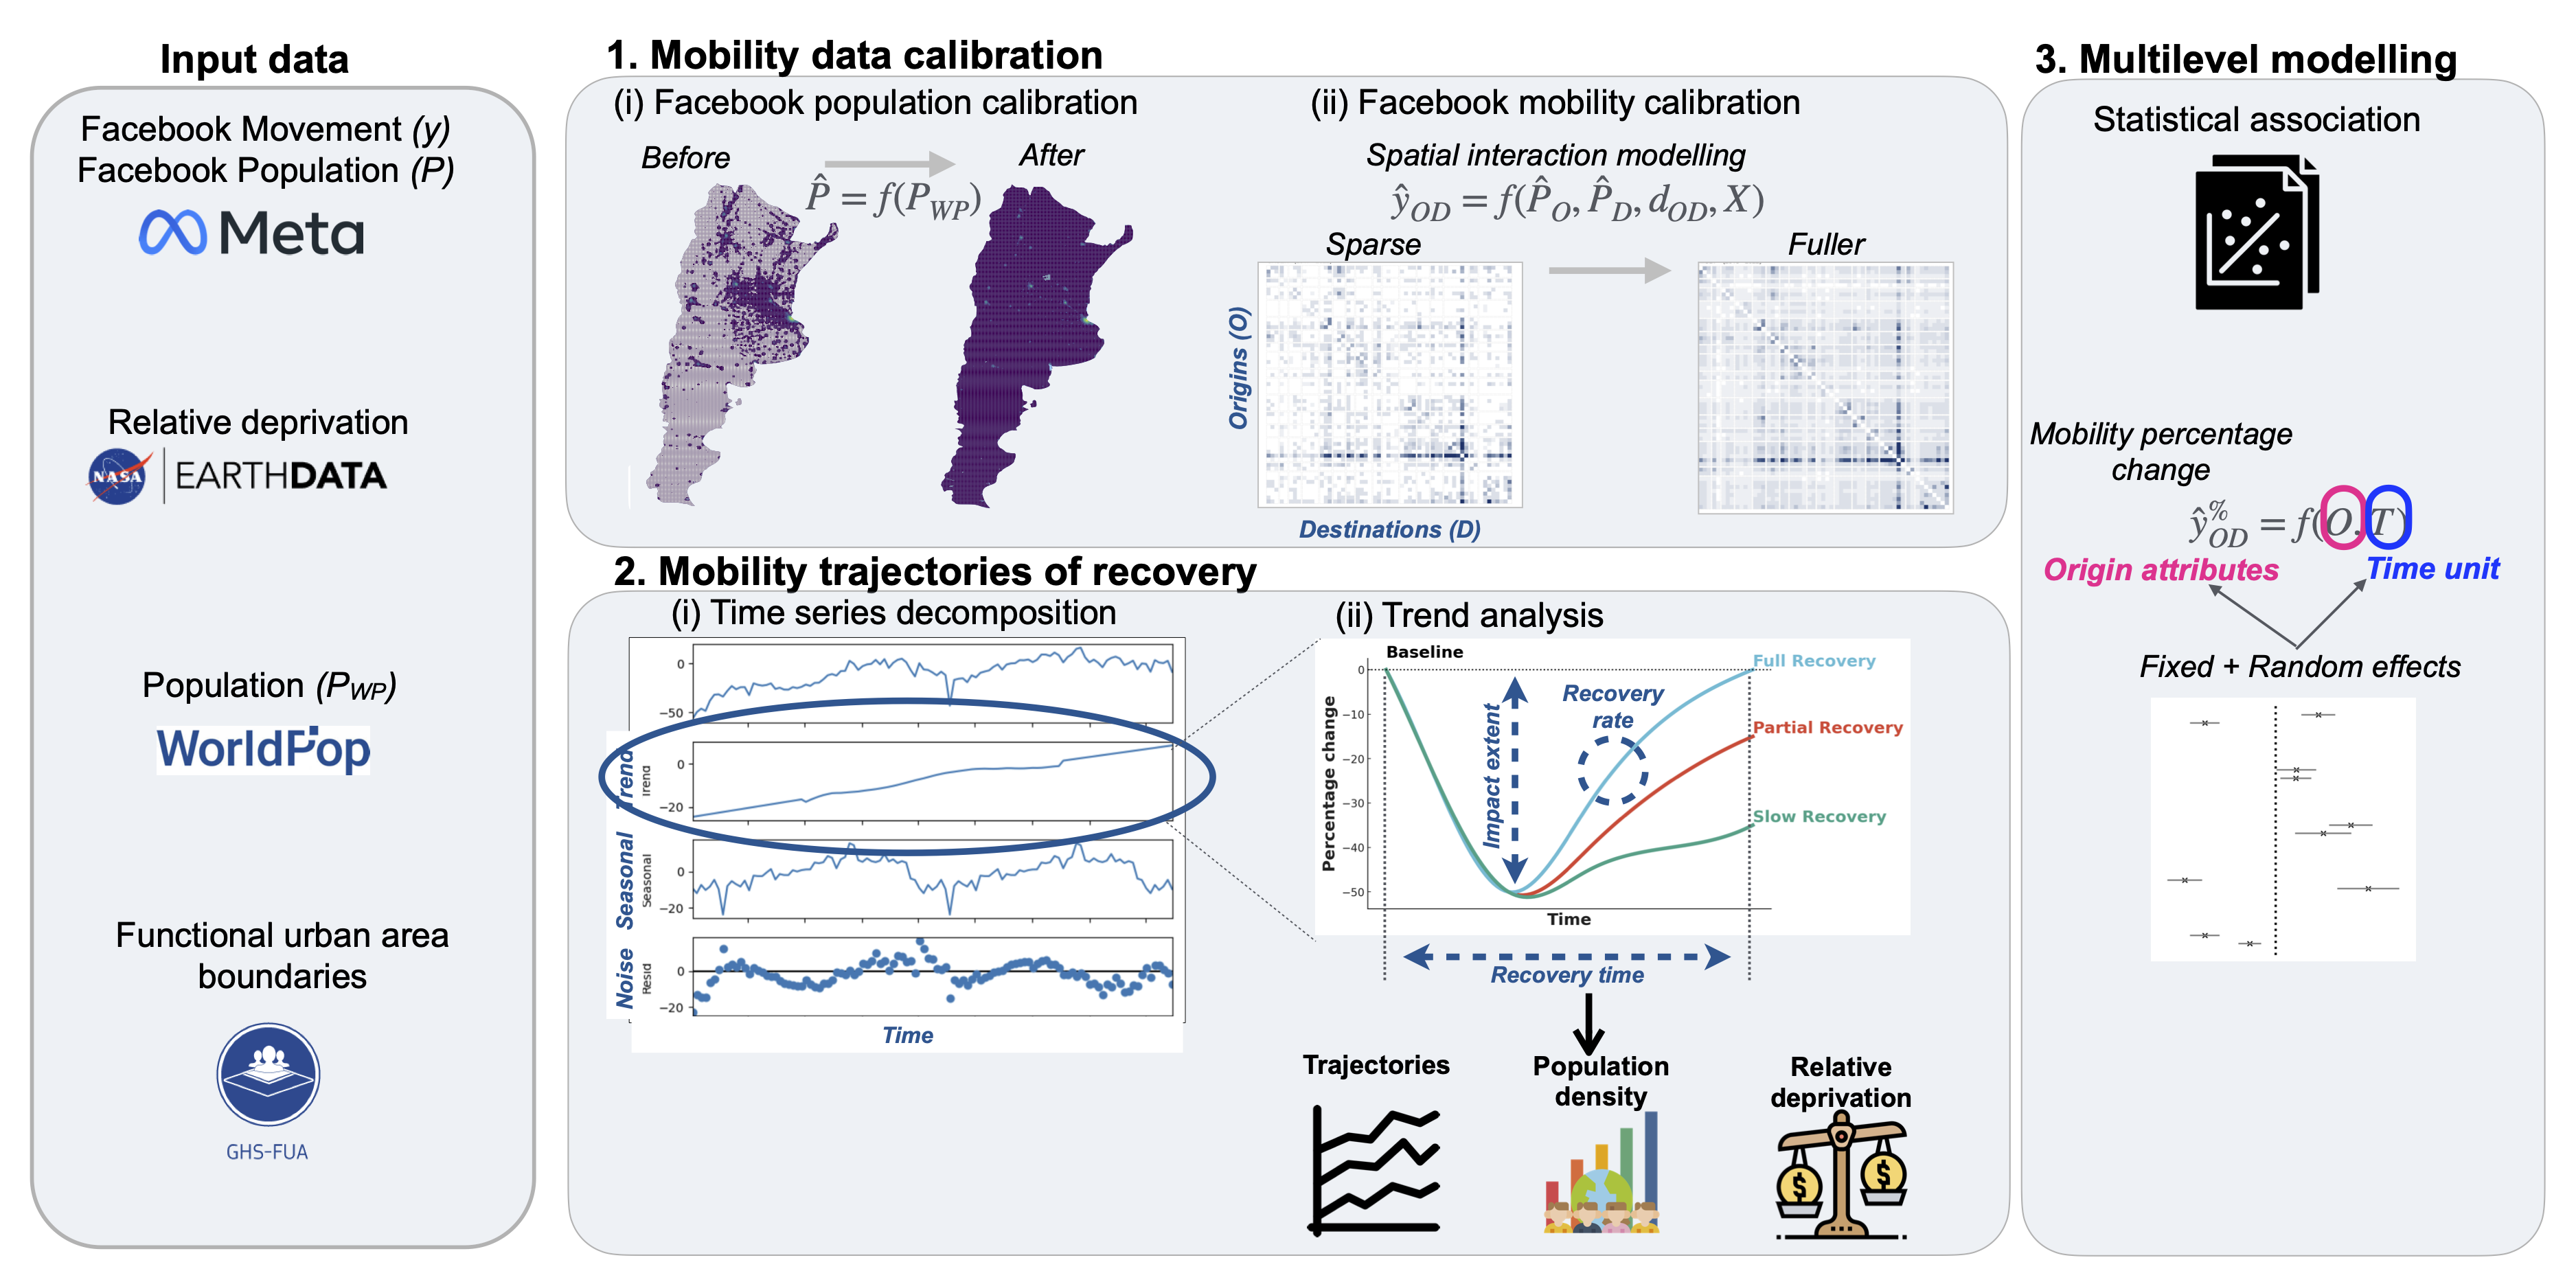
\includegraphics[width=\linewidth]{figures/Fig-summary-diagram.png}
%DIFDELCMD < %%%
\DIFdelendFL \DIFaddbeginFL 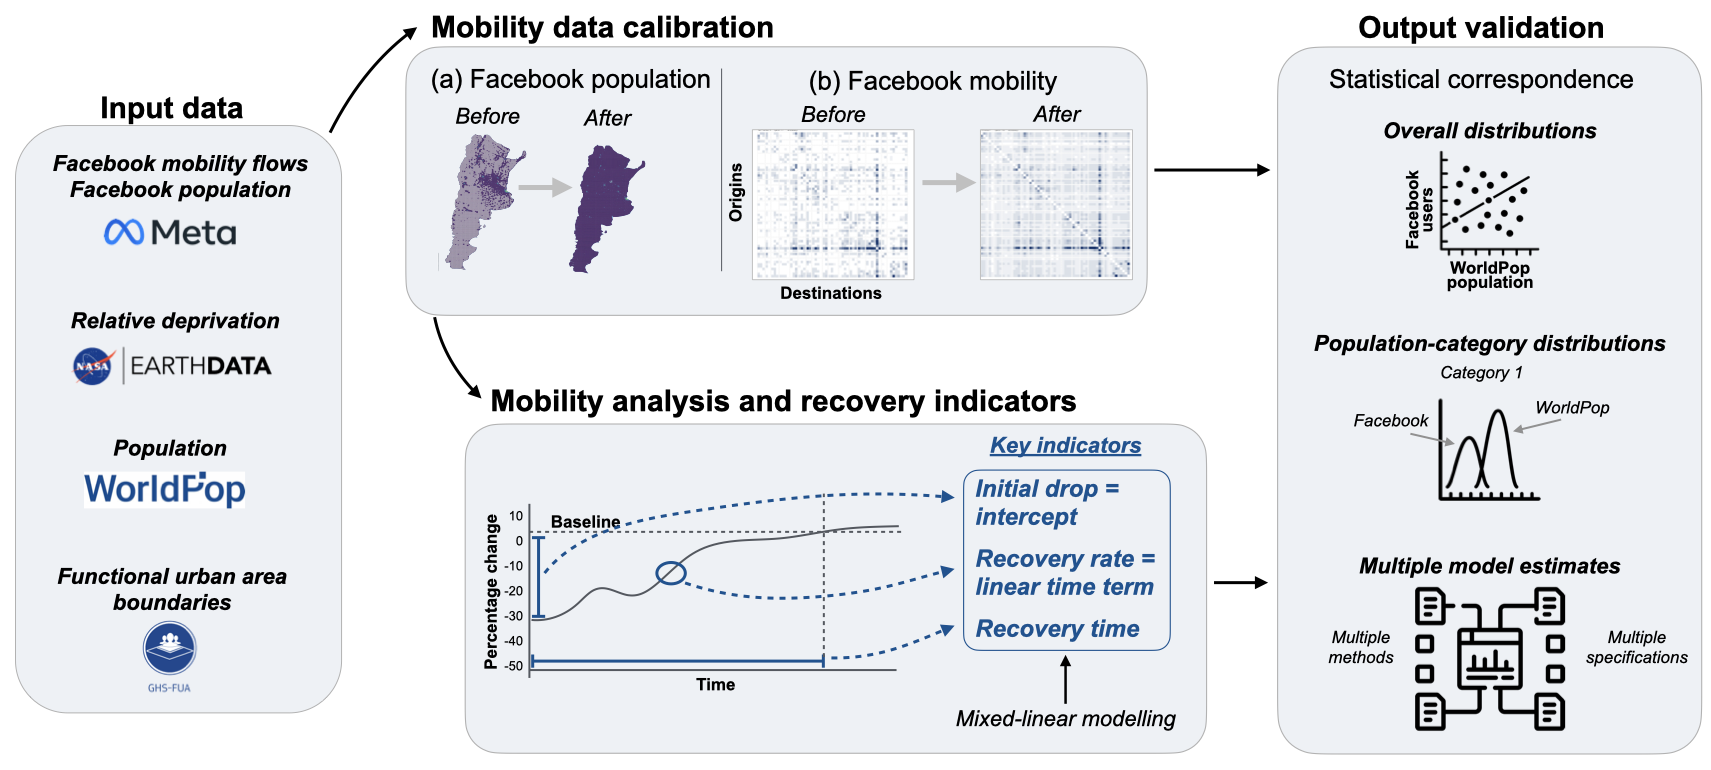
\includegraphics[width=0.9\linewidth]{figures/Fig-summary-diagram-r1.png}
\DIFaddendFL \caption{Overview of \DIFaddbeginFL \DIFaddFL{our methodology. Detailed descriptions are provided in the Methods section. Facebook mobility and population }\DIFaddendFL data \DIFdelbeginFL \DIFdelFL{input}\DIFdelendFL \DIFaddbeginFL \DIFaddFL{(Meta)}\DIFaddendFL , \DIFaddbeginFL \DIFaddFL{relative deprivation (NASA), population estimates (WorldPop) and functional urban area boundaries (Global Human Settlement Layer) are used as inputs. Mobility data are calibrated to reduce spatial and temporal biases and analysed within each country using statistical models to estimate urban mobility recovery. Validation assesses consistency with WorldPop populations and robustness across }\DIFaddendFL calibration and \DIFdelbeginFL \DIFdelFL{analysis}\DIFdelendFL \DIFaddbeginFL \DIFaddFL{model specifications}\DIFaddendFL .}
\label{fig-summary}
\end{figure}

We addressed important sources of common biases in mobile phone app data for our analysis. As most digital trace data, mobile phone data do not necessarily provide a representative picture of the overall population, largely because of algorithmic decisions and changes in users' engagement over time \DIFdelbegin \DIFdel{\mbox{%DIFAUXCMD
\cite{rowe2023big, barreras2024exciting}}\hskip0pt%DIFAUXCMD
}\DIFdelend \DIFaddbegin \DIFadd{\mbox{%DIFAUXCMD
\cite{rowe2023big, barreras2024exciting, cabrera2025bias}}\hskip0pt%DIFAUXCMD
}\DIFaddend . We know that Facebook suppresses population counts below 10 to protect users' privacy and that user engagement declined over time in our dataset. \DIFaddbegin \DIFadd{These adjustments may influence the observed patterns of mobility, especially in sparsely populated areas. }\DIFaddend To mitigate these issues, we applied a series of \DIFdelbegin \DIFdel{adjustments }\DIFdelend \DIFaddbegin \DIFadd{data corrections }\DIFaddend (see Figure \ref{fig-summary}). First, we modelled the Facebook user population data as a function of Worldpop population data to generate a complete spatial population surface. Second, we modelled the Facebook mobility data to estimate origin-destination flows that were suppressed by the Facebook algorithm. Third, we used the temporal median of the sum of active user counts divided by the sum of active user counts across all spatial units on a given day to normalise for fluctuations in Facebook user engagement over time. \DIFdelbegin \DIFdel{A full description }\DIFdelend \DIFaddbegin \DIFadd{Full details }\DIFaddend of these procedures \DIFdelbegin \DIFdel{is }\DIFdelend \DIFaddbegin \DIFadd{are }\DIFaddend provided in the Methods \DIFdelbegin \DIFdel{Section}\DIFdelend \DIFaddbegin \DIFadd{section, and ST1 summarises the extent of data imputation}\DIFaddend .

\subsection*{COVID-19 led to lasting disparities in mobility patterns}

We first compared the change relative to baseline levels of mobility during the early \DIFdelbegin \DIFdel{in the }\DIFdelend pandemic in 2020, and once most restrictions were lifted in 2022, as shown in Figure \ref{fig-impact}. Boxplots display the percentage change distribution of areas based on population density and relative deprivation level categories, with a $y = 0$ line representing baseline levels. Scores above this line indicate increased mobility from pre-pandemic levels, while values below represent a reduction. 

\begin{figure}[h!]
\centering
\DIFdelbeginFL %DIFDELCMD < 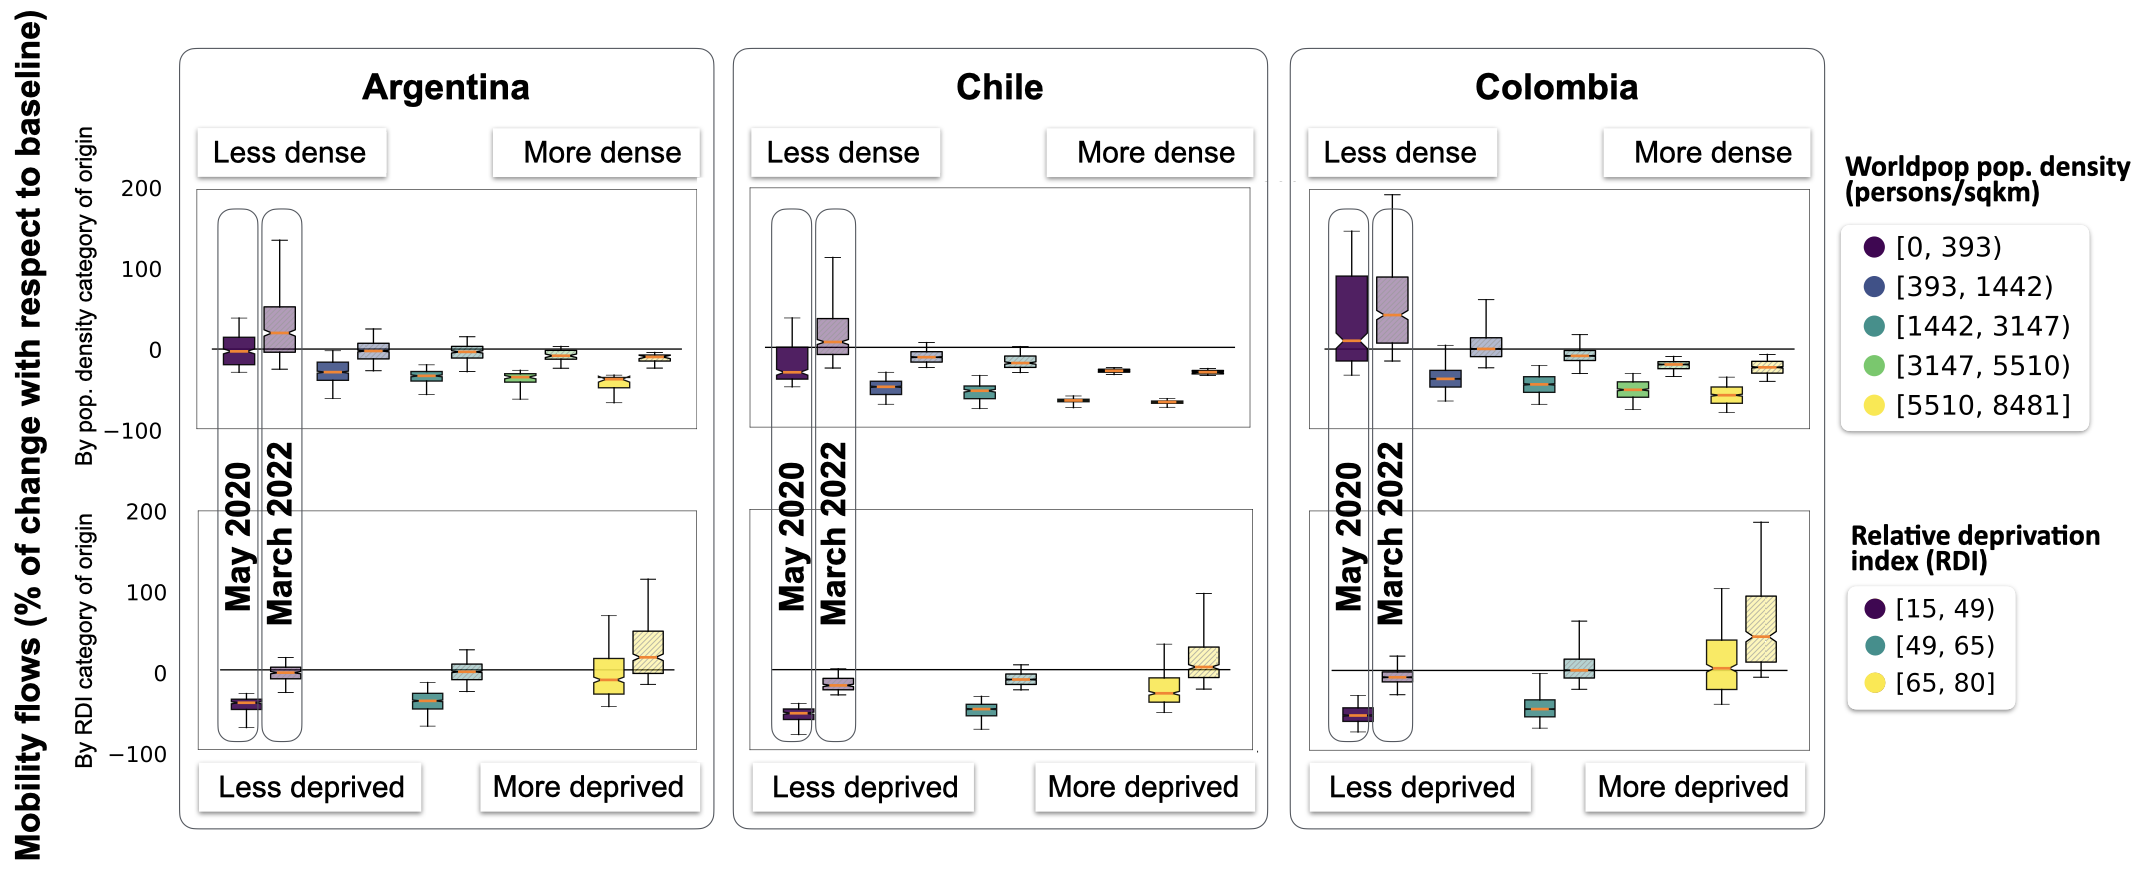
\includegraphics[width=\linewidth]{figures/Fig-impact-design.png}
%DIFDELCMD < %%%
\DIFdelendFL \DIFaddbeginFL 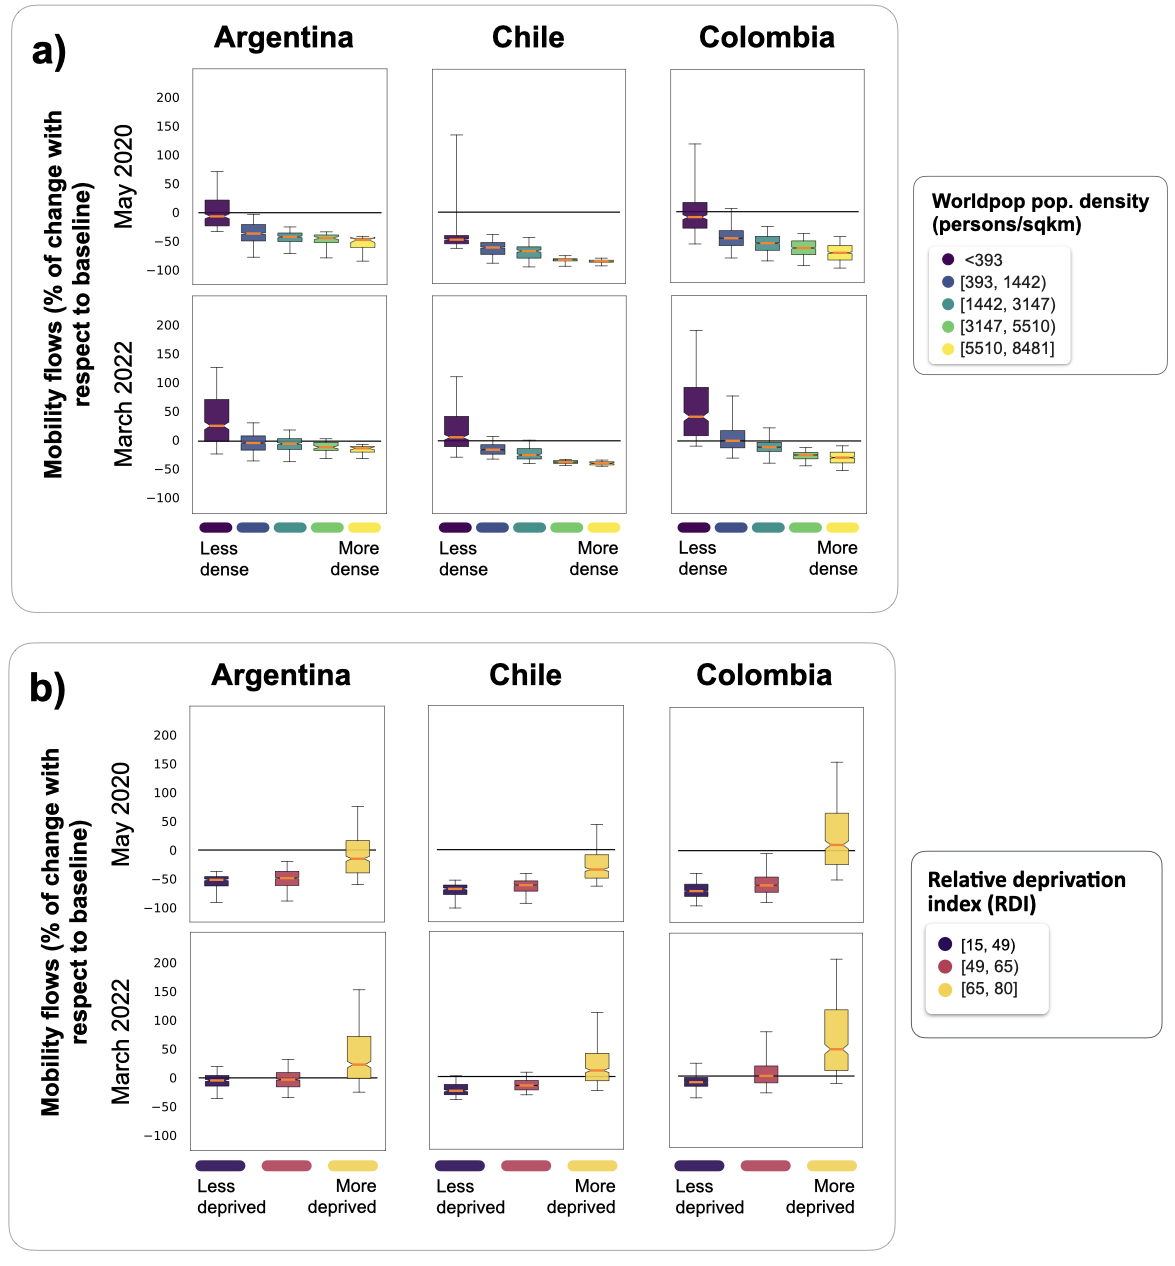
\includegraphics[width=0.9\linewidth]{figures/Fig-impact-design-r1.png}
\DIFaddendFL \caption{Percentage change in mobility counts in May 2020 and March 2022, relative to the pre-pandemic baseline levels, by population density category and deprivation index (RDI) category, Argentina, Chile and Colombia.}
\label{fig-impact}
\end{figure}

The results consistently show larger and more persistent declines in mobility in high-density areas compared to low-density areas. This persistence of reduced mobility levels in high-density areas is a novel finding, suggesting that the COVID-19 pandemic led to significant behavioural mobility changes in cities which have endured over time. The consistency of such a pattern is remarkable taking place in all three Latin American countries in our sample, showing little discrepancy within countries (as shown by relatively narrow box plots). In contrast, low-density areas show mobility patterns closer to pre-pandemic levels and greater variability. The large variability is due to the small population bases in these areas, where minor fluctuations in movement can result in disproportionately large percentage changes.

Our findings also evidenced enduring socio-economic disparities on the impact of the pandemic on mobility patterns. Prior research demonstrated that, early in the pandemic in 2020, a social gradient emerged, leading to sharper declines in mobility in less deprived areas compared to more deprived communities. We find that this social gradient effect has endured over time, as workers from more deprived areas are likely travelling as much (or more) as they used to prior to the outbreak of the COVID-19 pandemic - indicated by box plots stretching above baseline levels. These patterns are remarkably consistent across all three countries. This is despite differences in the initial extent of mobility decline across countries in 2020. Relative to baseline levels, initial reductions in mobility were larger in Chile (45-50\%) than in Colombia (40-45\%) and Argentina (25-30\%).


%DIF <  We generated time series of the percentage change in mobility flows relative to the baseline, covering the entire dataset period. Figure \ref{fig-recovery-combined} a) and b) shows this evolution, disaggregated by the population density and relative deprivation index category of the area where the outflow originates. Time is represented on the $x$-axis while the intensity of movement is depicted on the $y$-axis, measured as the percentage change in the number of outflows relative to pre-pandemic baseline levels. To provide context in the evolution of mobility levels over time, we colour the plot background using the stringency index, which quantifies changes in the level of COVID-19 non-pharmaceutical interventions, such as social distancing and lockdowns. The time series serve as input for the next stage of analysis, aimed at further characterising the disparities in the recovery of mobility.
\DIFdelbegin %DIFDELCMD < 

%DIFDELCMD < %%%
%DIF <  \begin{figure}[h!]
%DIF <  \centering
%DIF <  
\includegraphics[width=0.8\linewidth]{figures/Fig-recovery-combined-design.png}
%DIF <  \caption{Percentage change in outflows relative to pre-pandemic baseline levels in origin areas, for Argentina, Chile and Colombia, from mid-April 2020 to mid-April 2022: a) by population density category, b) by relative deprivation index (RDI) category.}
%DIF <  \label{fig-recovery-combined}
%DIF <  \end{figure}
%DIFDELCMD < 

%DIFDELCMD < %%%
\DIFdelend \subsection*{Early mobility declines during the pandemic shape long-term levels of mobility}

Discrepancies in the resilience of areas may underpin the observed differences in mobility levels. To quantify the resilience of areas, we model the trends of mobility recovery to pre-pandemic levels \DIFaddbegin \DIFadd{as a function of time}\DIFaddend . To this end, we decomposed the time series of the percentage change in mobility into trend, seasonal \DIFdelbegin \DIFdel{, }\DIFdelend and residual components \DIFdelbegin \DIFdel{based the Seasonal and Trend (STL) decomposition using Locally Estimated Scatterplot Smoothing (LOESS) \mbox{%DIFAUXCMD
\cite{cleveland1990stl}}\hskip0pt%DIFAUXCMD
}\DIFdelend \DIFaddbegin \DIFadd{using a moving-average–based method. Robustness checks using alternative trend extraction techniques are reported in Supplementary Table (ST) ST2}\DIFaddend . The time series are displayed in \DIFdelbegin \DIFdel{the SF9}\DIFdelend \DIFaddbegin \DIFadd{SF10}\DIFaddend . We modelled the trend component as a function of time, stringency levels and attributes of the places of origin, including population density\DIFdelbegin \DIFdel{and relative deprivation }\DIFdelend \DIFaddbegin \DIFadd{, relative deprivation and old-age dependency ratio (the latter category reported only in the Supplementary Information)}\DIFaddend , in a mixed-effects modelling framework – see Methods section and \DIFdelbegin \DIFdel{Supplementary Table (ST) 2 }\DIFdelend \DIFaddbegin \DIFadd{ST3 }\DIFaddend for details.  \DIFdelbegin \DIFdel{Fourteen different }\DIFdelend \DIFaddbegin \DIFadd{Stringency levels are measured via the COVID-19 Stringency Index created by \mbox{%DIFAUXCMD
\cite{hale2021global}}\hskip0pt%DIFAUXCMD
, which we include to assess the influence of changes in government restrictions on mobility. The index aggregates daily data on nine policy indicators including school and workplace closures, cancellation of public events, restrictions on gatherings and movement, public transport closures, stay-at-home requirements, international travel controls and public information campaigns. 
}

\DIFadd{Fourteen }\DIFaddend model specifications were fitted separately for each country. The full set of regression estimates \DIFdelbegin \DIFdel{are provided in ST3-8. Our stringency and time variables exhibited a strong negative correlation (Pearson correlation coefficient of -0.91, \mbox{%DIFAUXCMD
$p$
}%DIFAUXCMD
-value \mbox{%DIFAUXCMD
$< 0.01$
}%DIFAUXCMD
). Due to this high collinearity, the first and second rows of }\DIFdelend \DIFaddbegin \DIFadd{is provided in ST4-9. Time and stringency index were strongly colinear (Pearson \mbox{%DIFAUXCMD
$r = -0.91$
}%DIFAUXCMD
, \mbox{%DIFAUXCMD
$p < 0.01$
}%DIFAUXCMD
); accordingly, }\DIFaddend Figure \ref{fig-re-combined} (a) and (b) \DIFdelbegin \DIFdel{report parameter estimates from models that include only time as an explanatory variable (rather than both time and stringency). This decision is supported }\DIFdelend \DIFaddbegin \DIFadd{reports estimates from time-only models, which were also favoured }\DIFaddend by the Akaike Information Criterion (AIC)\DIFdelbegin \DIFdel{, which generally indicates better model fit (i.e. lower AIC scores) for time-only specifications}\DIFdelend . Among all models, Model 6 generally yields the lowest AIC score, indicating the best overall fit. \DIFaddbegin \DIFadd{To assess robustness, we additionally estimated a Generalised Additive Model (GAM) specification (Model 8). Although the GAMs consistently produced lower AIC values, they show evidence of overfitting (high effective degrees of freedom for class-specific splines). GAM model outcomes are also reported in ST4-9.
}\DIFaddend 

\DIFdelbegin %DIFDELCMD < \begin{figure}[H]
%DIFDELCMD < %%%
\DIFdelendFL \DIFaddbeginFL \begin{figure}[!htbp]
\DIFaddendFL \centering
\DIFdelbeginFL %DIFDELCMD < \includegraphics[width=\linewidth]{figures/Fig-re-combined-design-quad-recovery-time-std.png}
%DIFDELCMD < %%%
\DIFdelendFL \DIFaddbeginFL 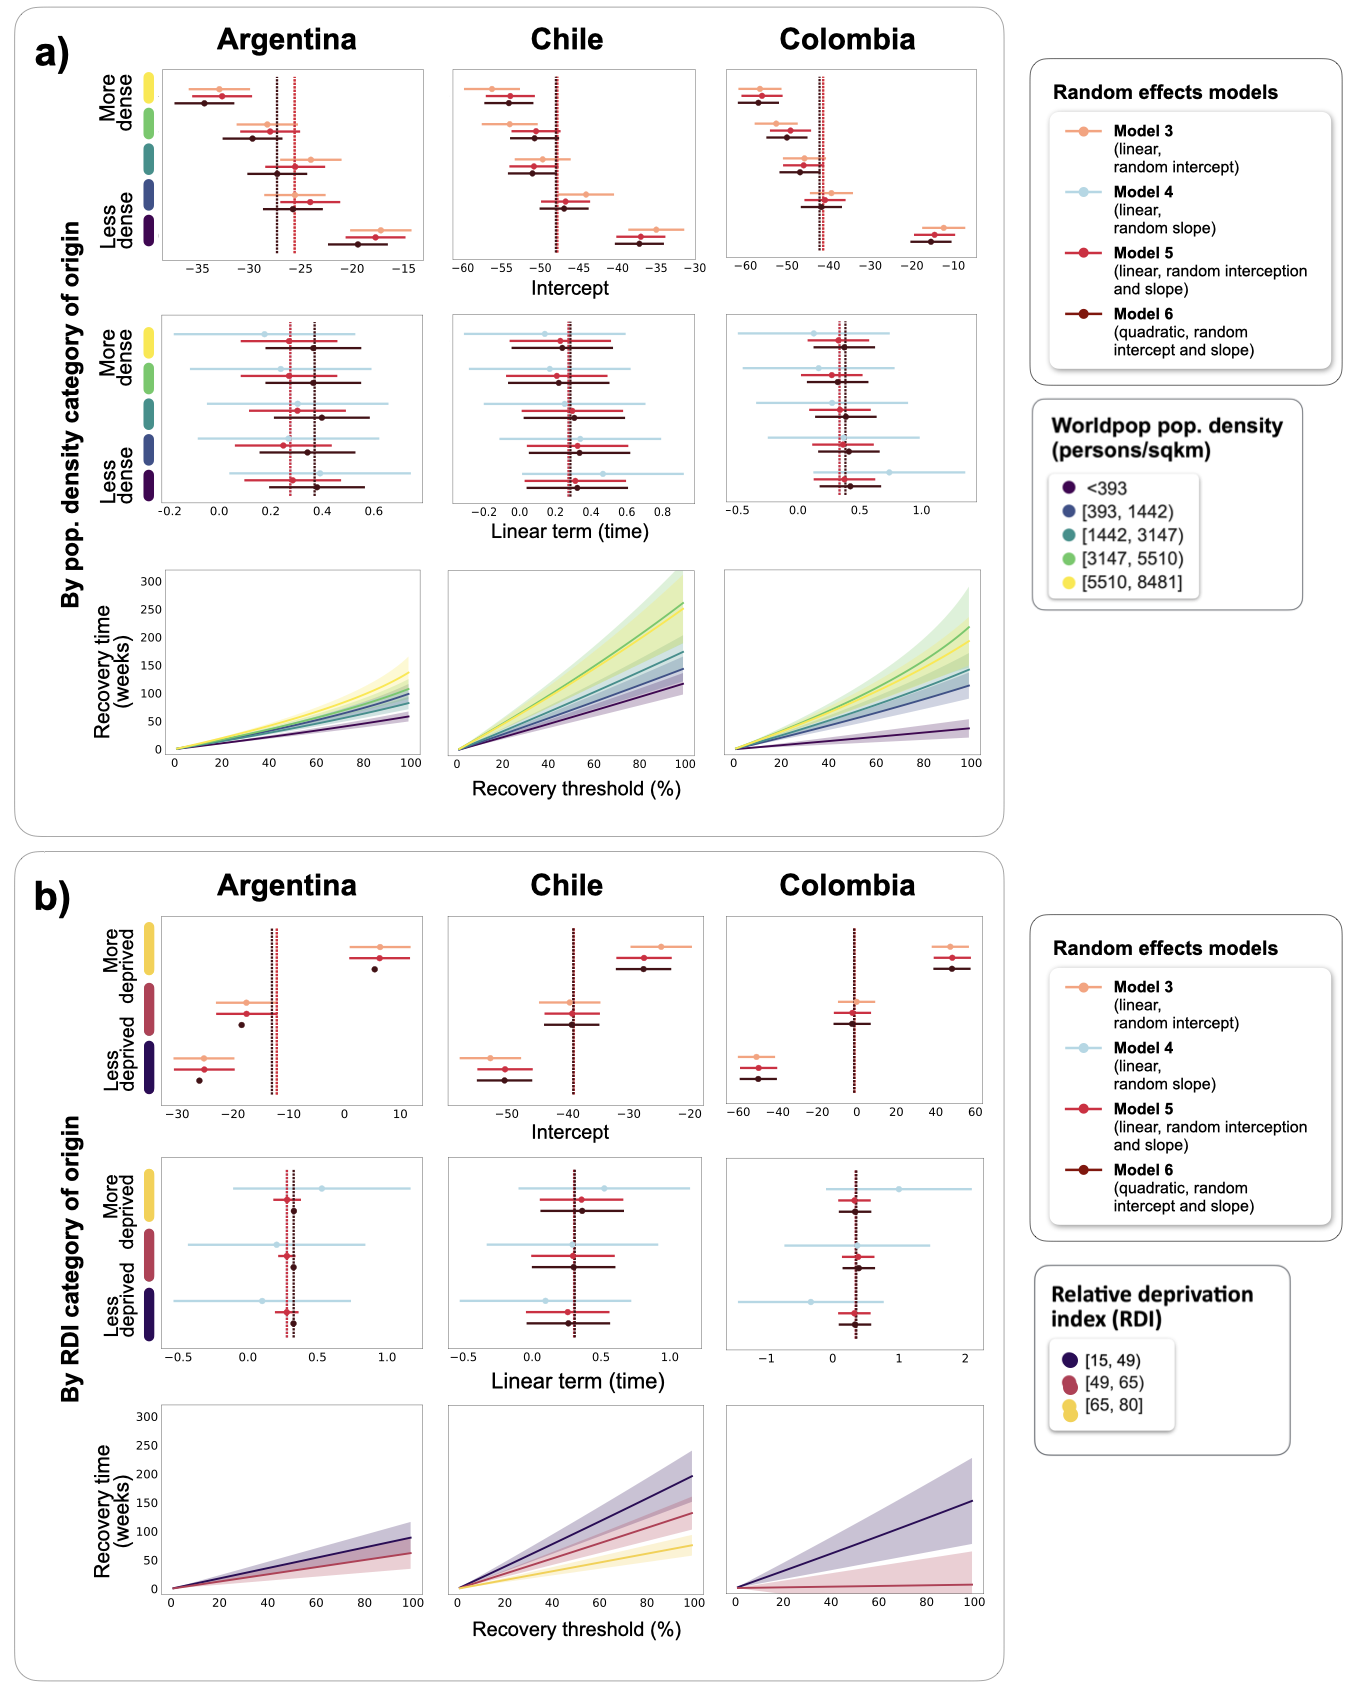
\includegraphics[width=0.9\linewidth]{figures/Fig-re-combined-design-quad-recovery-time-std-r1.png}
\DIFaddendFL \caption{First and second row of each panel represent mixed-effects modelling estimates (random intercept and random linear time term); bars denote 95\% confidence intervals; colours encode different model specifications; vertical dashed lines represent the estimated values for fixed effects of the corresponding terms (i.e. intercept, linear time). \DIFdelbeginFL \DIFdelFL{Third }\DIFdelendFL \DIFaddbeginFL \DIFaddFL{The third }\DIFaddendFL row represents estimated recovery times at different thresholds. Panel \DIFaddbeginFL \DIFaddFL{(}\DIFaddendFL a) displays results by population density category and \DIFaddbeginFL \DIFaddFL{(}\DIFaddendFL b) by relative deprivation category.}
\label{fig-re-combined}
\end{figure}

The model estimates reported in Figure \ref{fig-re-combined} correspond to coefficients for intercept and time terms from Models 3-6 for population density (a) and deprivation (b). The intercept represents the estimated percentage decline in mobility during the week when Meta began producing mobility records, correcting for seasonality and noise. Negative scores indicate reductions in mobility levels, relative to the baseline period. The time term captures the linear component of the weekly rate of mobility recovery, relative to baseline levels. A time quadratic term was also included to capture variations in the pace of mobility recovery over time as reported in \DIFdelbegin \DIFdel{ST3-8 }\DIFdelend \DIFaddbegin \DIFadd{ST4-9 }\DIFaddend for Models 6 and 7. Model 7 includes random effects for the quadratic term. This adds complexity to our model, but it does not improve the estimation (higher AIC) and is often insignificant (p-value$>0.05$). Estimates from various model specifications evidence the consistency of our findings. Additionally, we also estimated mobility recovery times, reported in both panels (a) and (b); that is, the time taken (in weeks) for mobility to reach various thresholds based on pre-pandemic mobility levels. For low-deprivation groups in Argentina and Colombia, recovery times are not reported, as average mobility levels for these groups did not fall below the baseline during the observation period. The Methods and Supplementary Information (SI, section 4) describe how the recovery time estimates and uncertainty bands were computed. \DIFdelbegin \DIFdel{ST21-24 }\DIFdelend \DIFaddbegin \DIFadd{ST22-23 }\DIFaddend report recovery time estimates by country at four different thresholds (25\%, 50\%, 75\% and 100\%), and by population density or RDI category\DIFdelbegin \DIFdel{.
}\DIFdelend \DIFaddbegin \DIFadd{, computed according to mixed-effects Model 6 and to GAM-based Model 8. 
}\DIFaddend 

\DIFdelbegin \DIFdel{First, our }\DIFdelend \DIFaddbegin \DIFadd{We highlight three main findings. First, the }\DIFaddend random intercept estimates \DIFdelbegin \DIFdel{is consistent with our }\DIFdelend \DIFaddbegin \DIFadd{are consistent with the }\DIFaddend evidence in Figure \ref{fig-impact} revealing a descending gradient across rural-urban and socioeconomic structures during early stages of the pandemic. Mobility declined the sharpest in highest-density and least-deprived areas, while low-density population and more deprived areas registered small declines. These estimates suggest that populations in affluent and more dense urban areas have more flexibility to adapt to early COVID-19 restrictions by reducing their mobility levels and turning to remote work. Poorer and less populated communities had less flexibility to transition to remote work. \DIFaddbegin \DIFadd{Although intercepts also differ across old-age dependency ratio categories, these differences do not form a systematic gradient across countries, so we only report them as part of the Supplementary Information (SF11; ST4–ST9).
}\DIFaddend 

Second, our regression estimates show differences in random intercepts \DIFdelbegin \DIFdel{and }\DIFdelend \DIFaddbegin \DIFadd{but }\DIFaddend overlapping confidence intervals for \DIFdelbegin \DIFdel{our }\DIFdelend \DIFaddbegin \DIFadd{the }\DIFaddend random time slopes. These results suggest that differences in mobility recovery across rural-urban and socio-economic gradients over time reflect differences in the magnitude of the initial mobility shock (intercepts), rather than in recovery rates (time slopes) following the initial COVID-19 outbreak. \DIFdelbegin \DIFdel{That is, the magnitude of the initial mobility shock tended to shape mobility recovery differences across rural-urban and socio-economic gradients. While the random slopes indicate no statistically significant difference in the rate of mobility recovery across rural-urban and socio-economic gradients. Yet, recovery }\DIFdelend \DIFaddbegin \DIFadd{Recovery }\DIFaddend time estimates indicate a consistent grading across rural-urban and socio-economic structures. Higher density and less deprived areas display longer recovery times, indicating that mobility is estimated to take longer to reach pre-pandemic mobility levels. Differences in recovery times along rural-urban and socio-economic gradients are \DIFaddbegin \DIFadd{therefore }\DIFaddend driven by the magnitude of the initial mobility shock (captured by our intercept estimates), rather than by differences in recovery rates (captured by our time estimates). \DIFaddbegin \DIFadd{These effects are similarly observed across old-age dependency ratio categories, as reported in SF11 and ST4-9.
}\DIFaddend 

Third, recovery time estimates (Figure \ref{fig-re-combined} bottom panel) indicate longer recovery periods in mobility for higher population density and less deprived areas. The lowest population density areas in Chile are estimated to take 132 weeks to achieve 100\% of observed pre-pandemic mobility levels, but \DIFdelbegin \DIFdel{only }\DIFdelend \DIFaddbegin \DIFadd{as much as }\DIFaddend 201.87 weeks in the highest density areas. The differences in recovery times are consistent across countries. Yet, wide variability exists between them. Chile systematically displays the longest estimated recovery times. They tend to be twice as large as those recorded for Argentina and Colombia, where stringency measures implemented at the outset of COVID-19 triggered a rise in mobility in the low density areas \DIFdelbegin \DIFdel{, }\DIFdelend and highly deprived communities, exceeding pre-pandemic levels (\DIFdelbegin \DIFdel{SF9}\DIFdelend \DIFaddbegin \DIFadd{SF10}\DIFaddend ).

Overall, our findings indicate \DIFdelbegin \DIFdel{that the degree of }\DIFdelend \DIFaddbegin \DIFadd{a strong }\DIFaddend persistence of the immediate \DIFdelbegin \DIFdel{shock of the }\DIFdelend COVID-19 \DIFdelbegin \DIFdel{pandemic on mobility levels}\DIFdelend \DIFaddbegin \DIFadd{mobility shock}\DIFaddend . They suggest that post-pandemic mobility disparities reflect the immediate shock of COVID-19, rather than differences in recovery rates across communities. COVID-19 appears to have led to new mobility regimes reflecting pre-existing urban and socio-economic inequalities. Our findings indicate that the unequal mobility declines observed in March 2020 across rural-urban and deprivation gradients persisted well beyond the lifting of restrictions and vaccine rollout, lasting at least two years after the onset of COVID-19.


%DIF < Next, we introduce a measure of recovery time based on Model 6, assuming a quadratic trend for the evolution of mobility levels relative to the baseline. The measure is fully defined in the Methods section. All values of recovery time at multiple thresholds are reported in Supplementary Table 21. We find that mobility recovery times in Argentina are relatively uniform across density categories, with full recovery ($t_{100}$) ranging from 69.81 to 105.79 weeks (approximately from 1 year and 4 months to 2 year and 1 month). Chile exhibits the longest recovery times, particularly in high-density areas, where $t_{100}$ reaches 201.87 weeks (approximately 3 years and 10 months). Colombia shows the fastest recovery among the three countries, especially in low-density areas, where $t_{100}$ is just 59.38 weeks (1 year and 2 month). Overall, higher population density is associated with longer recovery times, with this effect being most pronounced in Chile.
\DIFdelbegin %DIFDELCMD < 

%DIFDELCMD < %%%
%DIF < In Argentina, in higher deprivation areas it is not possible to compute recovery times, since mobility in these areas exceeded baseline levels from the start of the period of study. In contrast the less deprived areas record longer recovery times, indicating that the most affluent groups did not move as much as the most deprived. Chile shows a consistent pattern, with shorter recovery times in the most deprived areas (66.68 weeks for $t_{100}$, or 1 year and 4 months) and longer in less deprived areas (106.72 weeks for $t_{100}$, 1 year and 11 months). The patterns in Colombia are more mixed, with the medium-deprivation group showing negative recovery times. Generally, these results suggest that economic deprivation played a role in shaping mobility dynamics for all three countries, with Argentina and Chile clearly showing an earlier recovery of mobility in more deprived areas. 
%DIFDELCMD < 

%DIFDELCMD < %%%
\DIFdelend \subsection*{Dense urban cores report persistent reductions in net mobility outcomes}

Next\DIFaddbegin \DIFadd{, }\DIFaddend we examine the resilience of high-density urban core areas as attractors of daily mobility. Prior work identified a hollowing out of cities since the COVID-19 outbreak, or ``doughnut effect'', with a net loss of daily mobility into urban centres \cite{ramani2024working}. However, such evidence is limited outside the US context \cite{ramani2024working, gonzalez2023donut}. We analysed the evolution of netflows (i.e. inflows minus outflows) in relation to pre-pandemic levels. We measured netflows for all urban cores \DIFdelbegin \DIFdel{, or CBDs }\DIFdelend in the country, and only for the capital's urban core (i.e. Buenos Aires, Santiago and Bogotá), to assess the extent to which flows to the capital may influence the results. We used Functional Urban Areas (FUAs) boundaries from the GHSL to define urban regions \DIFdelbegin \DIFdel{as they delineate daily commuting activity spaces }\DIFdelend \cite{ceu.jrc.2019}, and for each urban region, we distinguish the urban core as the most densely populated spatial unit of analysis (the densest Bing tile within the FUA, see Methods), which effectively contains the CBD. 
%DIF < In Buenos Aires, only one of our Bing tiles is classified as a very high-density area (shown in yellow); hence, no exchanges are recorded between very high-density areas within the metropolitan area of Buenos Aires, and thus no reported in the first panel of 

Figure \ref{fig-fuasflows} displays the evolution of these netflows by population density category. We seek to assess the extent of \DIFdelbegin \DIFdel{loss population }\DIFdelend \DIFaddbegin \DIFadd{population loss }\DIFaddend in urban cores due to mobility and its durability since the onset of COVID-19. We evaluate if urban cores in Latin American countries recorded declines due to mobility redistributing people to moderate population density areas (suburbanisation); to low-density areas (counter-urbanisation); or both. In Argentina, only the area corresponding to the urban core in Buenos Aires is classified in the highest density category, so no mobility interactions with other high-density areas are captured when analysing just the capital's urban core; hence, no yellow curve for the first panel in Figure \ref{fig-fuasflows} is reported. We used a mixed-effects modelling framework to analyse the time series in Figure \ref{fig-fuasflows} and \DIFaddbegin \DIFadd{for robustness, we also used a GAM model (results reported in ST10-21). We then }\DIFaddend estimated recovery times at multiple thresholds\DIFdelbegin \DIFdel{(see ST9-20 and ST23-24). In some areas}\DIFdelend \DIFaddbegin \DIFadd{. These recovery times show remarkable consistency when estimated according to Model 6 and Model 8 (see 
ST24-25). According to our models}\DIFaddend , netflows to urban cores did not recover \DIFdelbegin \DIFdel{. As }\DIFdelend \DIFaddbegin \DIFadd{in some areas and as }\DIFaddend a result, recovery times could not be estimated for \DIFdelbegin \DIFdel{these areas(ST9-20 and ST23-24)}\DIFdelend \DIFaddbegin \DIFadd{those areas}\DIFaddend .

%When the baseline netflow is positive, a negative percentage change between -100\% and 0\% indicates that the netflow decreases compared to the baseline but remains positive. Conversely, when the baseline netflow is negative, a percentage change between -100\% and 0\% suggests that the netflow remained negative during the crisis, though its absolute value was smaller than in the baseline period.

\begin{figure}[h!]
\centering
\DIFdelbeginFL %DIFDELCMD < 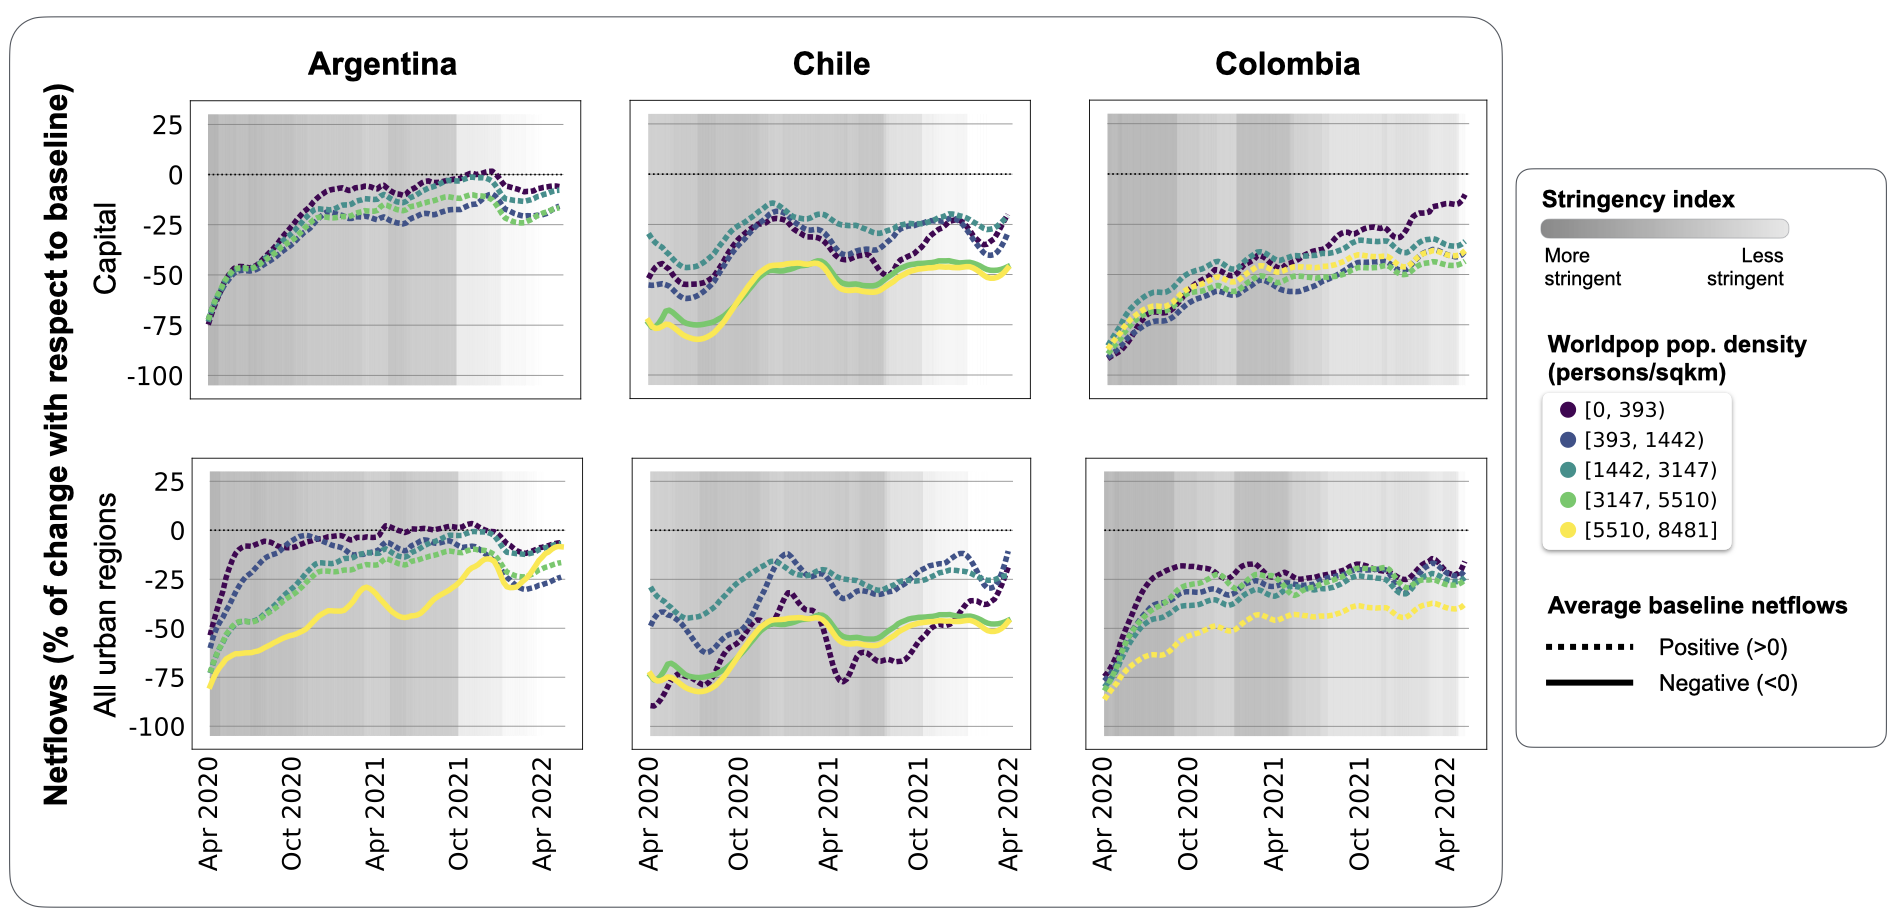
\includegraphics[width=\linewidth]{figures/Fig-fuas-netflows-simpler-no-baseline.png}
%DIFDELCMD < %%%
\DIFdelendFL \DIFaddbeginFL 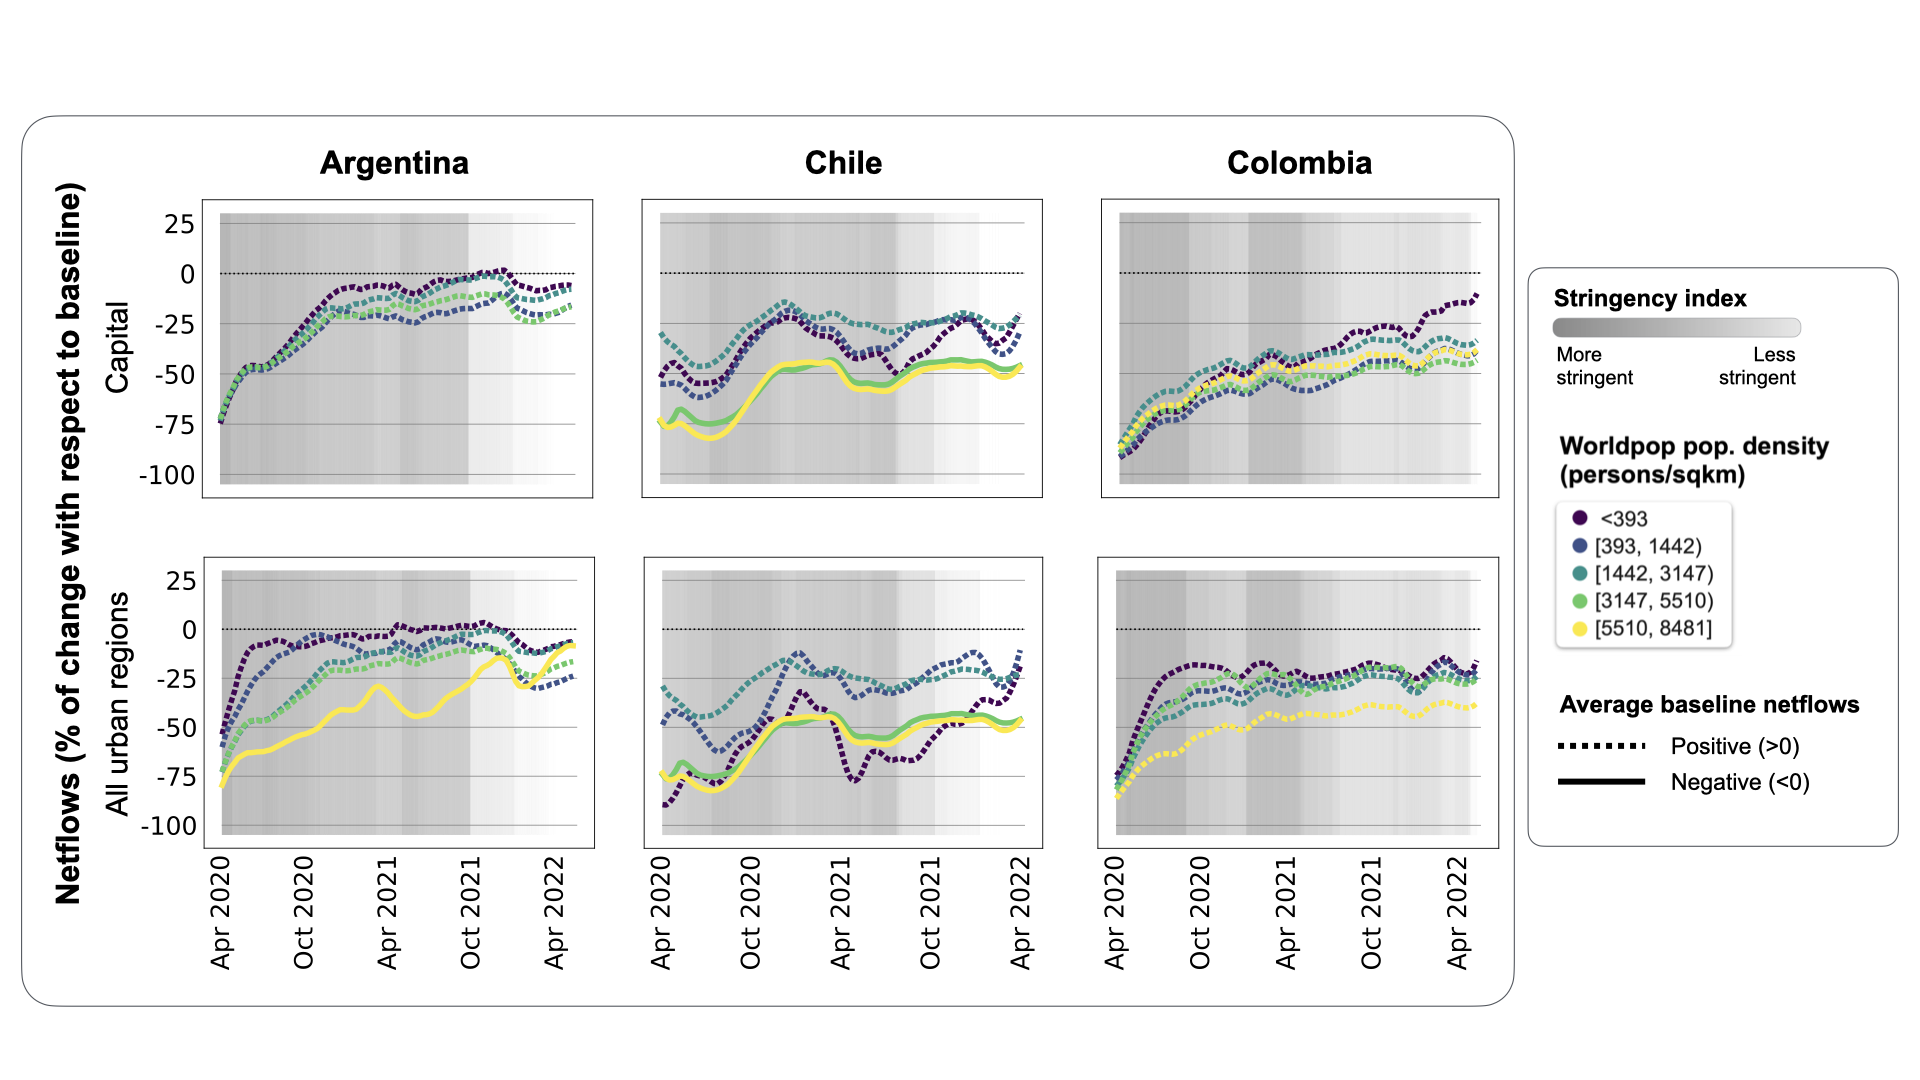
\includegraphics[width=\linewidth]{figures/Fig-fuas-netflows-simpler-no-baseline-r1.png}
\DIFaddendFL \caption{Evolution of netflows for urban cores corresponding to the capital urban region and all urban regions (defined as Functional Urban Areas), by population density category for Argentina, Chile and Colombia, April 2020 to May 2022. Netflows are expressed relative to pre-pandemic baseline levels. Dashed and solid lines indicate, respectively, positive or negative pre-pandemic netflows on average.}
\label{fig-fuasflows}
\end{figure}

Our findings suggest a prevalent pattern of reduced netflows for urban cores following the enforcement of COVID-19 restrictions. Dashed lines indicate that netflows in urban cores incoming from other areas were positive pre-pandemic. However, the negative relative change since the COVID-19 outbreak reveals a reduction in the magnitude of these netflows. This reduction has predominantly become less acute over time across the rural-urban hierarchy in all three countries, but it remained below pre-pandemic levels following the lifting of COVID-19 restrictions in May 2022. These patterns reflect that while mobility inflows into core areas continued to exceed outflows, they shrank resulting in a smaller net balance. In Argentina and Chile, particularly in the capital city of Buenos Aires and Santiago, patterns of negative netflows are consistent with systematic evidence of net population losses due to internal migration in these metropolitan centres over the last two decades \cite{rowe2013spatial, vignoli2019efectos, rodriguez2022migracion}.


%DIF < We model the trend component of the time series in \ref{fig-fuasflows}. Assuming the quadratic model in equation \eqref{model-trend}, we estimate recovery times for netflows according to equation \eqref{recovery-time-formula} (all values reported in Supplementary Tables 22-23). We observe that in many cases, mobility never reaches baseline levels, particularly in urban areas from Chile. Netflows between the capital's urban core and the less densely populated areas within the surrounding urban region tend to return to baseline levels more quickly. This is likely due to the fact that residents in these areas rely more on high-density urban cores for essential daily activities.
\DIFdelbegin %DIFDELCMD < 

%DIFDELCMD < %%%
%DIF < The patterns observed in high-density urban cores across all urban regions are similar to those found in capital cities. However, netflows between urban cores and less densely populated areas within urban regions tend to rebound more quickly toward pre-pandemic levels than when considering only the capital. This initial rebound is followed by a stabilisation of the percentage change, and netflows seem to never return to normal. This pattern further suggests that urban cores have lost some of their appeal, even among nearby low-density areas that may have previously been more dependent on them.
%DIFDELCMD < 

%DIFDELCMD < %%%
\DIFdelend \section*{Discussion}

%DIF <  I am getting a sense that we are saying that mobility is a sign of vulnerability: low-density and highest deprived areas - lower GDP country display closer mobility levels to prepandemic and faster recovery times. Would be good to look for literature on this. I can think of how mobility levels evolve with development, and there is a stage, they do grow with development before decreasing as areas become more developed.
\DIFdelbegin %DIFDELCMD < 

%DIFDELCMD < %%%
\DIFdel{Using Meta-Facebook origin-destination mobility data derived from GPS mobile phone locations, we }\DIFdelend \DIFaddbegin \DIFadd{We }\DIFaddend assessed the durability of changes in mobility patterns across rural–urban and socio-economic gradients in Latin American countries \DIFdelbegin \DIFdel{during }\DIFdelend \DIFaddbegin \DIFadd{from }\DIFaddend the beginning of the pandemic outbreak in March 2020 and following the rollout of vaccines and relaxation of lockdown measures in May 2022. Prior work showed that the pandemic resulted in large reductions in mobility levels in high-density urban areas and least deprived communities, reflecting reductions in commercial activity in urban areas, and a higher representation of affluent communities in jobs with higher potential for remote working \cite{bartik2020jobs}. Yet, existing evidence has focused on the immediate impacts of COVID-19 during early 2020 and on the restructuring of mobility patterns in more developed countries. We contribute to expanding this work by investigating the evolving impacts of COVID-19 on mobility beyond their initial aftermath extending to the second year of the pandemic in less developed countries.

We find evidence of sustained reductions in mobility levels in high-density urban areas and among the least deprived communities. These declines, first observed in the early months of the COVID-19 pandemic, persisted two years later, despite widespread vaccine rollout and the lifting of lockdown measures. We also find a sustained reduction of net balance of mobility flows in core urban areas. Historically, cities are critical engines of innovation, economic growth and prosperity \cite{Glaeser10}, enabling the emergence of agglomeration economies and facilitating knowledge exchange \cite{storper2004}. Our findings suggest that some of these benefits may have diminished. COVID-19 accelerated the adoption of technologies, online services and remote working at an unprecedented scale, reducing the need for physical co-location and eroding the vibrancy of urban centres \cite{Alexander21}. As people engage in virtual activities, planning strategies should be reoriented to repurpose existing infrastructure and develop new required infrastructure, \DIFdelbegin \DIFdel{to accommodate }\DIFdelend \DIFaddbegin \DIFadd{accommodating }\DIFaddend the ways in which people move and use cities in a post-pandemic world. Transport systems, for example, may need to be redesigned to accommodate less frequent trips to core urban areas, and less frequent but \DIFdelbegin \DIFdel{long-distance }\DIFdelend \DIFaddbegin \DIFadd{longer-distance }\DIFaddend commuting trips from \DIFdelbegin \DIFdel{less dense areas locations }\DIFdelend \DIFaddbegin \DIFadd{lower-density areas }\DIFaddend to employment centres. Digital infrastructure in more remote areas may require an upgrade to accommodate improved connectivity and seamless virtual data transfers.

\DIFdelbegin \DIFdel{Importantly, our }\DIFdelend \DIFaddbegin \DIFadd{Our }\DIFaddend findings reveal persistent differences in mobility recovery trends across rural-urban and socio-economic gradients. We find that disparities in the initial impact of the COVID-19 pandemic on mobility across population groups largely account for the sustained differences in recovery trajectories. \DIFdelbegin \DIFdel{Notably, while }\DIFdelend \DIFaddbegin \DIFadd{While }\DIFaddend the magnitude of the initial shock varied significantly across rural-urban and socio-economic groups, the subsequent rates of mobility recovery have remained relatively uniform over the long term. Higher-density and less deprived areas \DIFdelbegin \DIFdel{display }\DIFdelend \DIFaddbegin \DIFadd{displayed }\DIFaddend shorter overall recovery times compared to lower-density and more deprived areas. \DIFdelbegin \DIFdel{These disparities reflect }\DIFdelend \DIFaddbegin \DIFadd{Disparities in mobility are likely driven, to a great extent, by }\DIFaddend differences in the nature of employment \cite{ILO21} \DIFaddbegin \DIFadd{across rural-urban and socio-economic groups, }\DIFaddend and \DIFdelbegin \DIFdel{can arguably enhance pre-existing socioeconomic inequalities, as daily mobility entails financial and non-financial opportunity costs, such as transport fares and travel time, which may disproportionally burden the most disadvantaged communities. Pandemic-induced differences in mobility behaviour across deprivation groups may }\DIFdelend \DIFaddbegin \DIFadd{may }\DIFaddend continue in the future if current remote work practices are maintained. However, \DIFdelbegin \DIFdel{they }\DIFdelend \DIFaddbegin \DIFadd{these patterns }\DIFaddend may be about to change following recent shifts in employers' attitudes towards remote working, such as the presidential actions of the US government, with mandates for more days in the office \cite{WhiteHouse2025Return, CIPD2025LMO}. Overall, our findings suggest that \DIFaddbegin \DIFadd{government }\DIFaddend efforts to reduce mobility disparities across rural-urban and deprivation divides should prioritise mitigating the initial shock of pandemics, as recovery trajectories tend to progress at similar rates across groups once the immediate disruption has passed.

\DIFdelbegin \DIFdel{In Latin America, }\DIFdelend \DIFaddbegin \DIFadd{Despite our robustness and validation tests, key challenges should be considered when interpreting our results. First, limitations related to the use of aggregated mobile-phone–derived mobility indicators. These data are generated from a non-random sample of users providing variable coverage across space and time, and potentially under-representing population groups with lower smartphone access, limited digital connectivity or higher privacy opt-out rates \mbox{%DIFAUXCMD
\cite{cabrera2025bias}}\hskip0pt%DIFAUXCMD
. As such, inferred mobility changes may not fully reflect the behaviour of all sociodemographic groups, particularly in more disadvantaged areas. Second, the pre-pandemic baseline used to define reference mobility levels is limited to a 45-day period provided by Meta and therefore does not capture longer-term seasonal variability. While this baseline precedes mobility restrictions and accounts for day-of-week effects, it may affect estimates of the absolute magnitude of the initial mobility drop, though relative recovery trajectories are less sensitive to this limitation. Third, our data do not provide information on modal split, limiting inference on the persistence of changes in specific transport modes, such as walking or cycling \mbox{%DIFAUXCMD
\cite{zhang2023impacts}}\hskip0pt%DIFAUXCMD
. Fourth, observed mobility changes reflect outcomes rather than travel motivations, constraining our ability to distinguish behavioural adaptation from mobility reductions driven by affordability, service availability or labour informality. Finally, our analyses are observational and conducted at an aggregate spatial scale, so associations between mobility recovery and city characteristics should not be interpreted as causal and may be influenced by unobserved factors, such as changes in transport supply or concurrent economic shocks. These limitations motivate future work combining digital trace mobility data with external validation sources and complementary data to assess representativeness, modal shifts and causal mechanisms.
}

\DIFadd{The evidence reported here potentially has important social equity implications by exacerbating pre-existing disparities in Latin America. The region is among }\DIFaddend the \DIFdelbegin \DIFdel{implications of our findings are specially serious, as the sustained pandemic-induced changes that we observed in mobility may exacerbate existing large levels of inequality. Latin America is considered one of the }\DIFdelend most unequal regions in the world \cite{WIReport22}. The bottom 50\% \DIFdelbegin \DIFdel{holding only }\DIFdelend \DIFaddbegin \DIFadd{of the Latin American population holds only around }\DIFaddend 10\% of \DIFdelbegin \DIFdel{the national wealthin the region will probably face a greater relative social burden induced by their }\DIFdelend \DIFaddbegin \DIFadd{wealth\mbox{%DIFAUXCMD
\cite{WIReport22}}\hskip0pt%DIFAUXCMD
, and is likely to face a disproportionately high social burden due to a more }\DIFaddend limited capacity to work remotely \DIFdelbegin \DIFdel{. At the same time}\DIFdelend \DIFaddbegin \DIFadd{and a continued reliance on physical mobility for accessing employment and services. This entails financial and non-financial opportunity costs, such as transport fares and travel time. By contrast}\DIFaddend , the top 10\% \DIFdelbegin \DIFdel{holding }\DIFdelend \DIFaddbegin \DIFadd{of the population, which holds approximately }\DIFaddend 55\% of \DIFdelbegin \DIFdel{the national wealth}\DIFdelend \DIFaddbegin \DIFadd{wealth\mbox{%DIFAUXCMD
\cite{WIReport22}}\hskip0pt%DIFAUXCMD
, }\DIFaddend may continue to \DIFdelbegin \DIFdel{travel less often to urban centres, reducing their footprint, commercial activity in these areas, and eventually their overall vibrancy. If intensified and sustained, these trends will amplify already visible }\DIFdelend \DIFaddbegin \DIFadd{reduce travel due to greater flexibility in work arrangements and access to digital alternatives. As a result, uneven mobility recovery across socio-economic groups may function as a mechanism through which pandemic-era disruptions become embedded into long-standing patterns of inequality and spatial mismatches between residence and opportunity, with potential consequences for labour market participation, educational attainment and access to essential services. 
}

\DIFadd{These sustained mobility changes also have important implications for Latin American cities and their governance. Sustained suppression of mobility into urban cores risks undermining commercial activity and overall urban vibrancy, particularly if higher-income populations continue to travel less frequently to central areas. These dynamics may reinforce already emerging }\DIFaddend patterns of urban centre \DIFdelbegin \DIFdel{decay }\DIFdelend \DIFaddbegin \DIFadd{decline }\DIFaddend in some large Latin American cities, as we saw in European cities during the 1970s and 1980s \cite{THORSTEN}. \DIFaddbegin \DIFadd{In Latin America, where metropolitan governance is often fragmented across municipalities and fiscal capacity for large-scale interventions remains limited \mbox{%DIFAUXCMD
\cite{un2022world, inostroza2013urban, fay2017rethinking, irazabal20governance}}\hskip0pt%DIFAUXCMD
, the persistence of depressed urban core activity highlights the need for targeted, context-specific responses, rather than broad calls for inclusive or sustainable mobility. Policies prioritising affordable and reliable public transport connections to central employment and service hubs, particularly during peak hours and along high-demand corridors, may be more effective than uniform system-wide measures \mbox{%DIFAUXCMD
\cite{rivas2019urban, guzman2022effects}}\hskip0pt%DIFAUXCMD
. More broadly, the observed heterogeneity in recovery trajectories underpins the importance of metropolitan-scale coordination in transport and urban planning, as city-level responses alone may be insufficient to address persistent shifts in urban activity patterns \mbox{%DIFAUXCMD
\cite{duque2021institutional}}\hskip0pt%DIFAUXCMD
. In this scenario, near real-time mobility data offer a valuable tool for identifying emerging signals of urban decline and supporting adaptive, evidence-based policy interventions in contexts where traditional data sources remain delayed or incomplete.
}\DIFaddend 


% Key points to get across
%    - Although diminished, the early reduction in mobility in highly dense urban areas and the least deprived continued after two years the initial COVID-19 outbreak
%        - Implications: hibrid working and 
%    - The initial gap in reductions in mobility levels across the rural-urban and deprivation structures has persisted over time, reflecting limited differences in the rate of mobility recovery and longer recovery times in highly dense urban areas and less deprive communities.
%        - Looking at future recovery
%    - Net flows in core urban areas have systematically reduced and remained below pre-pandemic levels.
%        - Implications in terms of loss of attractiveness / hibrid working / more sustainable cities. 
%    - Methodological contribution on calibrating the data, correcting for biases



% Assuming a linear trend in mobility recovery, we find that highly dense urban areas take up to 2.5 times longer to recover than sparsely populated areas. In sparsely populated areas, mobility recovered faster as residents rely on travel to access essential services, reflecting that movement is a necessity rather than a choice. Similarly, deprived areas tend to recover faster than affluent areas, with the former sometimes experiencing little to no decline in mobility. More deprived populations are likely to work in occupations that require in-person presence, leaving them with fewer opportunities for remote work. Affluent populations, on the other hand, are more likely to hold office-based jobs that allow for remote work, reducing the immediate need to resume regular movement \cite{ILO21}.

% Our findings indicate that the resilience of different areas to the impact of the pandemic is mainly determined by the severity of the initial shock, rather than differences in their recovery rate. Since the recovery rate (slope of linear trend) is similar across population groups, all areas followed parallel recovery trajectories once mobility began rebounding. However, areas that experienced a more severe initial decline (intercept) had a longer road to recovery because they started from a lower point. This suggests that strengthening resilience to shocks such as pandemics requires strategies that minimise the severity of the initial impact, as recovery patterns tend to follow a similar trajectory across different areas. 

% Two years after the initial outbreak, daily movement into urban cores has not fully recovered in most cases, with a particularly sharp decline in Chile. The advantages of agglomeration economies, which include fostering innovation and growth by clustering talent and resources \cite{storper2004}, have historically driven urban resilience, particularly in the context of pandemics \cite{Glaeser10}. However, COVID-19 has accelerated the adoption of technologies that reduce the need for physical co-location at an unprecedented scale \cite{Alexander21}. As more people engage in virtual activities such as remote work, online shopping or digital collaboration, there is a need to rethink planning, infrastructure, and economic strategies to sustain urban vitality in a post-pandemic world.

\section*{Methods}

\subsection*{Data}

\subsubsection*{Facebook Movement During Crisis}

We used anonymised aggregate mobile phone location data from \DIFdelbegin \DIFdel{Facebook-Meta }\DIFdelend \DIFaddbegin \DIFadd{Meta-Facebook }\DIFaddend users to capture population movements for Argentina, Colombia and Chile, covering a \DIFdelbegin \DIFdel{24-month }\DIFdelend \DIFaddbegin \DIFadd{26-month }\DIFaddend period from April 2020 to \DIFdelbegin \DIFdel{March }\DIFdelend \DIFaddbegin \DIFadd{May }\DIFaddend 2022. We used the Facebook Movement During Crisis datasets created by Meta and accessed through their Data for Good Initiative (\href{https://dataforgood.facebook.com}{https://dataforgood.facebook.com}). The data are built from Facebook app users who have the location services setting \DIFdelbegin \DIFdel{turned on on }\DIFdelend \DIFaddbegin \DIFadd{activated on }\DIFaddend their smartphone. Prior to releasing the datasets, Meta ensures privacy and anonymity by removing personal information and applying three privacy-preserving processes \cite{Maas19}. First, Meta adds a small, undisclosed amount of random noise to prevent the determination of precise counts for these areas.
Second, they apply spatial smoothing, using inverse distance-weighted averaging, to create a smoother data surface. Third, they drop small counts to exclude records data counts below 10.

The Facebook Movement datasets provide information on the aggregated number of Facebook app users moving between pairs of locations from April 2020 to \DIFdelbegin \DIFdel{March }\DIFdelend \DIFaddbegin \DIFadd{May }\DIFaddend 2022 during the COVID-19 crisis period. The data is spatially aggregated into tiles according to the Bing Maps Tile System developed by Microsoft \cite{MicrosoftBingMaps}. The Facebook Movement data are spatially aggregated into Bing tiles at resolution level 10 for Argentina and Chile, and level 12 for Colombia, which correspond to squares of 19.57 $\times$ 19.57 km \DIFdelbegin \DIFdel{, }\DIFdelend and 4.89 $\times$ 4.89 km, respectively. The data are temporally aggregated into three daily 8-hour time windows which are 00:00-08:00, 08:00-16:00 and 16:00-00:00, Pacific Time (PT).
These time windows translate to 05:00-13:00, 13:00-21:00, 21:00-05:00 for Argentina and Chile; and 03:00-11:00, 11:00-19:00, 19:00-03:00 for Colombia. For each time window, the origin location of a user is defined as the most frequently visited location in the previous time window, while the destination location is the most frequently visited location in the relevant time window.

%DIF < We filtered the data to include only the morning time window for two reasons. First, this period is most likely to capture the majority of commuter activity. Second, focusing only on one part of the day avoids potential cancellation effects that could arise from considering all daily trips, as individuals typically engage in a round-trip pattern (e.g., travelling from home in the morning and returning in the evening). 
\DIFdelbegin %DIFDELCMD < 

%DIFDELCMD < %%%
\DIFdelend In addition, each dataset includes baseline movement counts, which represent the estimated number of people moving before COVID-19. These baseline counts \DIFaddbegin \DIFadd{provided by Meta }\DIFaddend are calculated based on a 45-day period ending on March 10, 2020, using the average for the same time of day and day of the week within this period. For example, \DIFaddbegin \DIFadd{Meta calculates }\DIFaddend the baseline for the 00:00–08:00 (PT) window on Mondays \DIFdelbegin \DIFdel{is calculated }\DIFdelend by averaging all Monday records for that time window across the 45-day period. Further details about the baseline can be found in \cite{Maas19}.

Due to the small-count dropping privacy measure, movement counts during both the crisis and baseline periods are excluded if they fall below 10. However, even when counts are not reported, the datasets consistently provide the percentage change in movement counts relative to the baseline. This percentage change, denoted as $y^{\%}_{ijdt}$, is computed as follows \cite{Maas19}:

\begin{equation}
y^{\%}_{ijdt} = \dfrac{y^{c}_{ijdt} - y^b_{ijdt}}{y^b_{ijdt} - \varepsilon}\times 100.
\end{equation}

Here, $y^c_{ijdt}$ and $y^b_{ijdt}$ represent the crisis and baseline movement counts, respectively, between origin tile $i$ to destination tile $j$ on day $d$ and during time window $t$. For the baseline values $y^b_{ijwt}$, the subindex $w$ denotes the day of the week corresponding to day $d$, as the baseline values are recorded by weekday, not by specific date. A small constant $\varepsilon$, usually set to 1, is added to the denominator to avoid division by zero \cite{Maas19}.

\subsubsection*{Facebook Population During Crisis}

We also used the Facebook Population During Crisis datasets. Like the Facebook Movement data, these datasets cover a \DIFdelbegin \DIFdel{24-month }\DIFdelend \DIFaddbegin \DIFadd{26-month }\DIFaddend period from April 2020 to \DIFdelbegin \DIFdel{March }\DIFdelend \DIFaddbegin \DIFadd{May }\DIFaddend 2022 and provide information on the number of active Facebook users at specific locations during the crisis period. The Facebook Population data for Argentina, Chile and Colombia are spatially aggregated into Bing tiles at resolution level 11 for Argentina and Chile, and level 12 for Colombia, which correspond to 9.78 $\times$ 9.78 km and 4.89 $\times$ 4.89 km tiles respectively. The Facebook Population data is aggregated temporally into 8-hour time windows. A user's location is defined as the most frequently visited location within each 8-hour time window.
Similar to the Facebook Movements datasets, the \DIFdelbegin \DIFdel{Populations }\DIFdelend \DIFaddbegin \DIFadd{Population }\DIFaddend datasets include baseline counts, calculated by averaging values for the same day of the week and time of day over the 45-day pre-pandemic baseline period\DIFdelbegin \DIFdel{provided by Meta}\DIFdelend .

The same privacy-preserving techniques are applied to the Facebook Population datasets.
As a result, population counts during both the crisis and baseline periods are excluded if they fall below 10. However, the datasets consistently report the percentage change in active user counts relative to the baseline. For tile $i$, day $d$ and time window $t$, the relative change in active user counts $p^{\%}_{idt}$ is computed as:

\begin{equation}
   p^{\%}_{idt} = \dfrac{p^{c}_{idt} - p^b_{iwt}}{p^b_{iwt} - \varepsilon}\times 100, 
\end{equation}

where $p^c_{idt}$ and $p^b_{iwt}$ represent the crisis and baseline active user counts at tile $i$ on day $d$ and during time window $t$. Once again, the subindex $w$ in baseline values $p^b_{iwt}$ denotes the day of the week corresponding to day $d$, and $\varepsilon$ is a small constant usually set to 1, added to the denominator to avoid division by zero \cite{Maas19}. \DIFdelbegin %DIFDELCMD < 

%DIFDELCMD < %%%
\DIFdel{We }\DIFdelend \DIFaddbegin \DIFadd{Through the paper, we }\DIFaddend use the term ``Facebook population'' in reference to the number of active Facebook app users.

\subsubsection*{Meta-Facebook data pre-processing}

We only included Facebook data for one time window per day: 08:00–16:00 Pacific Time (PT) corresponding to 13:00–21:00 in Argentina and Chile, and 11:00–19:00 in Colombia.
This time window is used to capture daily \DIFdelbegin \DIFdel{commutes}\DIFdelend \DIFaddbegin \DIFadd{mobility}\DIFaddend . Including data for the three time windows in the datasets could result in movement in opposite directions cancelling out \DIFdelbegin \DIFdel{and precluding us to capture }\DIFdelend \DIFaddbegin \DIFadd{when aggregating by day, and preventing us from capturing }\DIFaddend any meaningful patterns. To reflect our focus on one time window, we can drop the subindex $t$.

As a pre-processing step, we ensure that both the Facebook movement and population data are aligned in terms of spatial resolution for each country. Since the Facebook Population datasets are available at a finer spatial resolution, we re-aggregate them to match the spatial resolution of the Facebook Movement data.

\subsubsection*{Worldpop population data}

We used data from Worldpop \cite{tatem2017} to classify our spatial units by population density category \DIFdelbegin \DIFdel{, and }\DIFdelend \DIFaddbegin \DIFadd{and to }\DIFaddend estimate missing baseline values in the Facebook population data.
We used gridded population data at a resolution of 1km$^2$ in raster format. We performed a spatial join of the Facebook spatial units (Bing tiles) with the gridded population data and computed the sum of Worldpop populations corresponding to each of the Facebook spatial units. \DIFaddbegin \DIFadd{In addition, we used the age-disaggregated WorldPop layers to compute the old-age dependency ratio in each spatial unit (defined as the percentage of the population aged 65 and over), which we used to examine differences in mobility patterns by age structure. The results of this analysis by age structure are reported in the Supplementary Information.
}\DIFaddend 

\subsubsection*{Socioeconomic deprivation data} 

We used the Global Gridded Relative Deprivation Index (GRDI), Version 1 (GRDIv1) \cite{RDI2022} dataset as a measure of socioeconomic deprivation.
The GRDI data is available via NASA's Socioeconomic Data and Applications Centre (SEDAC) at a spatial resolution of 30 arc-seconds, or 1 km$^2$ approximately.
The index quantifies the relative levels of multidimensional deprivation and poverty, where a value of 100 represents the highest level of deprivation and a value of 0 the lowest.
We performed a spatial join of the Facebook spatial units and the gridded relative deprivation data. We computed the average RDI corresponding to each of the Facebook spatial units.


\DIFaddbegin \subsection*{\DIFadd{Addressing missing data through data imputation}} 

\DIFaddend A challenge in analysing the Facebook population counts and movements is the absence of records for small counts. These records are removed to ensure privacy and anonymity. Yet, they may impact the analysis as the Facebook datasets include a high \DIFdelbegin \DIFdel{proportion }\DIFdelend \DIFaddbegin \DIFadd{number }\DIFaddend of missing records, as shown in ST1\DIFdelbegin \DIFdel{, and missingness is not at random in these datasets}\DIFdelend . Missing values display a strong spatial pattern (see SF1). As such, sparsely populated spatial units \DIFdelbegin \DIFdel{, }\DIFdelend or small active Facebook user \DIFdelbegin \DIFdel{population }\DIFdelend \DIFaddbegin \DIFadd{populations }\DIFaddend could potentially be under-represented in the analyses. Simply removing the missing records from the analysis could lead to geographically biased results \cite{afghari2019}. To address this, we designed a data processing method for missing data imputation. \DIFdelbegin \DIFdel{An overview of this data imputationmethod is provided in Figure \ref{fig-dataimputation}.
}\DIFdelend \DIFaddbegin \DIFadd{After imputation, the alignment between Facebook-derived population distributions and WorldPop benchmarks improves, particularly across population density and deprivation categories (see SF8), indicating that the corrected data offer a more representative input for subsequent mobility analyses.
}\DIFaddend 

\begin{figure}[h!]
\centering
\DIFdelbeginFL %DIFDELCMD < 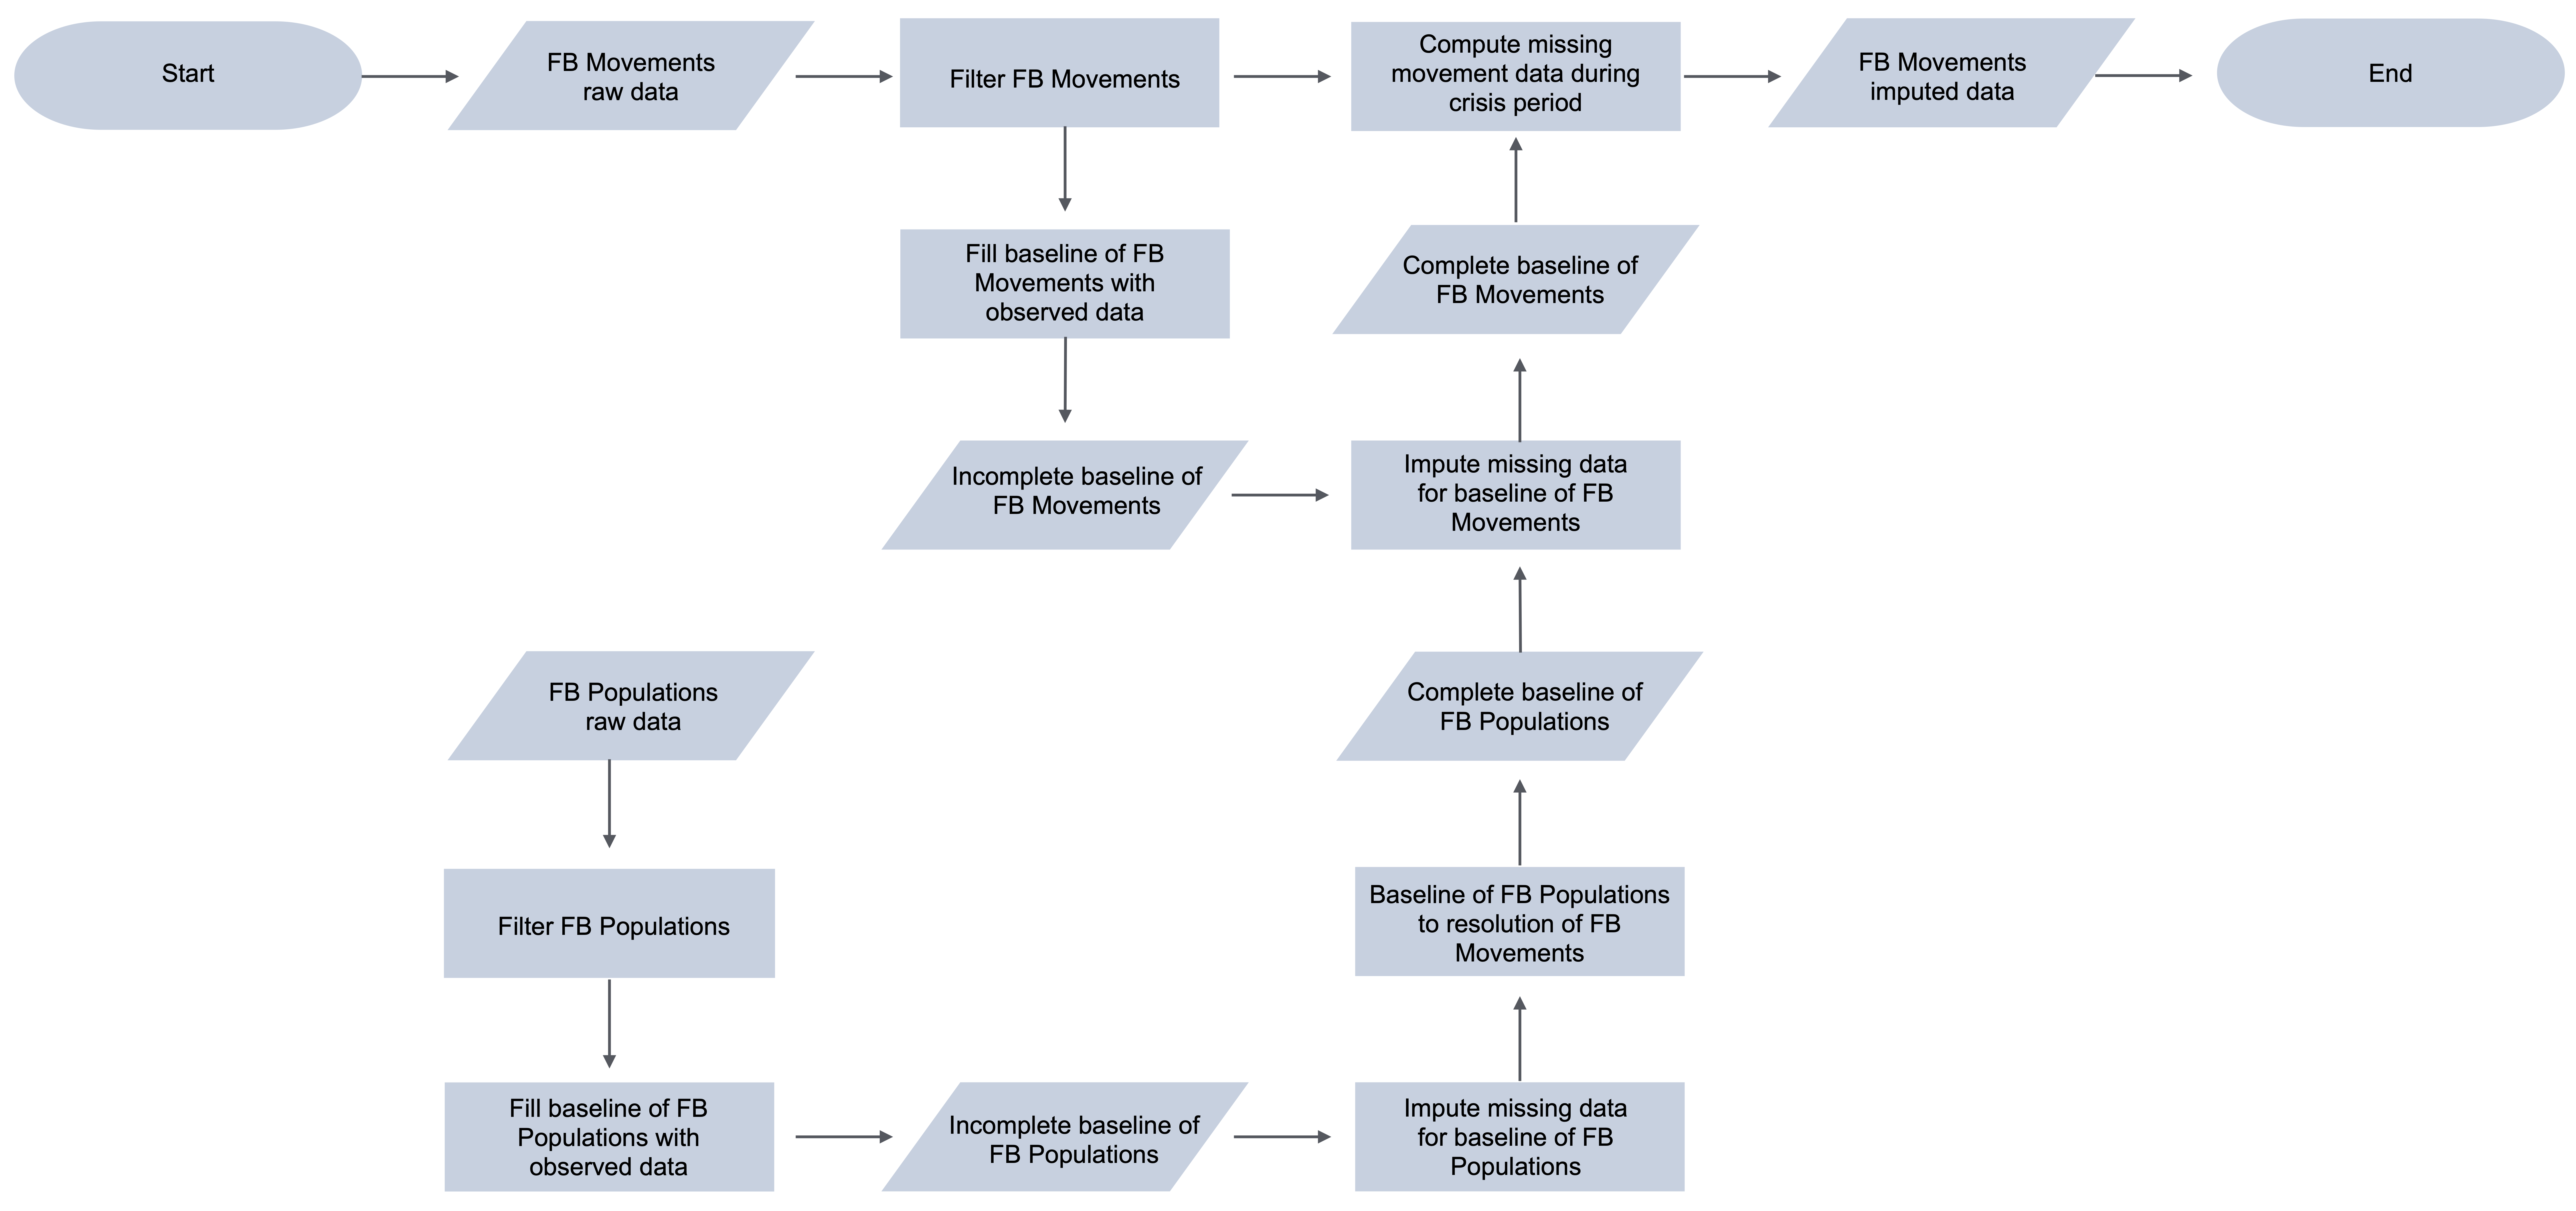
\includegraphics[width=\linewidth]{figures/workflow-diagram.png}
%DIFDELCMD < %%%
%DIFDELCMD < \caption{%
{%DIFAUXCMD
\DIFdelFL{Workflow diagram for data imputation method.}}
%DIFAUXCMD
\DIFdelendFL \DIFaddbeginFL 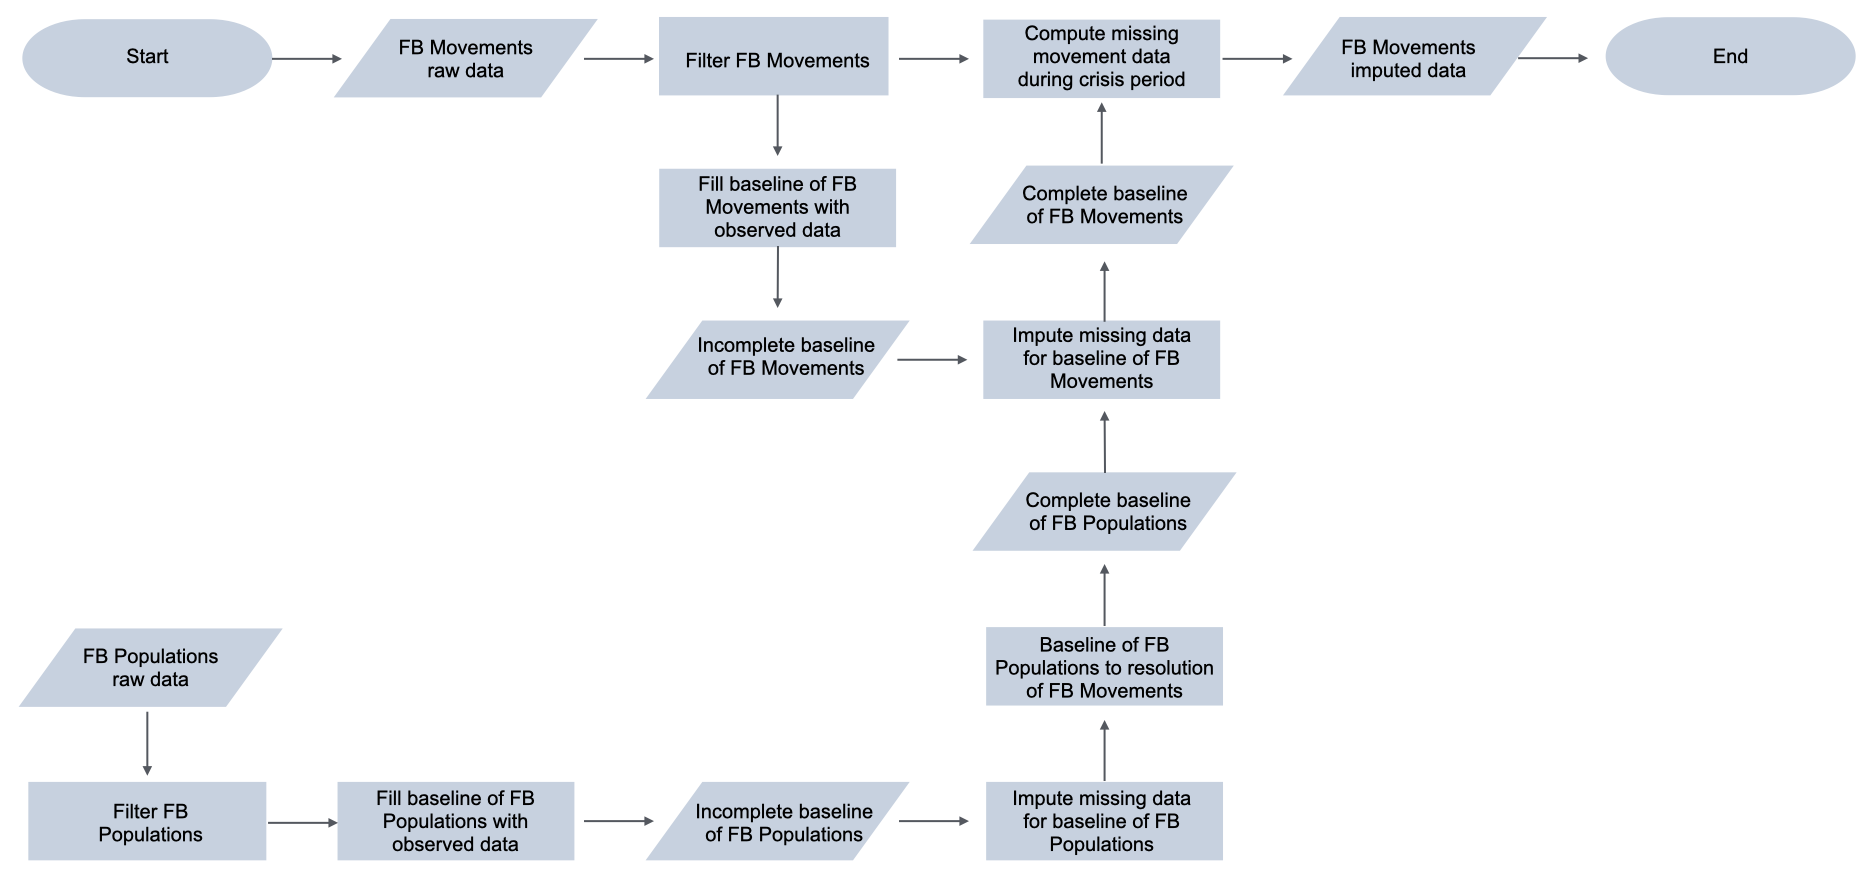
\includegraphics[width=\linewidth]{figures/workflow-diagram-r1.png}
\caption{\DIFaddFL{Workflow diagram for the data imputation method. Rectangular boxes represent processes or actions, rhomboid shapes indicate inputs or outputs, and oval shapes mark the start and end of the workflow.}}
\DIFaddendFL \label{fig-dataimputation}
\end{figure}

\DIFdelbegin \DIFdel{Additionally, we address a second challenge which is changes in the number of active Facebook users over time. To address this, we applied correction factors and time series smoothing to eliminate the fluctuations in the daily number of observations, ensuring that the representativeness of Facebook data across spatial units remains stable during the study period.
The steps of our data-processing workflow are described next.
}\DIFdelend \DIFaddbegin \subsubsection*{\DIFadd{Imputing Facebook Population data}}
\DIFaddend 

\DIFdelbegin \subsection*{\DIFdel{Imputing Facebook Population data}}
%DIFAUXCMD
%DIFDELCMD < 

%DIFDELCMD < %%%
\DIFdelend First, we identified all the baseline values reported in the Facebook Population datasets, which form the basis for creating a new dataset that includes all available baseline information. Following \cite{duan2024}, we used linear models to estimate the missing Facebook population baseline counts based on Worldpop population data. These models are fitted using ordinary least squares regression, with Worldpop data as the explanatory variable and the available baseline counts from the Facebook Population dataset as the dependent variable. The estimation process and its accuracy are illustrated in SF2-4 for Argentina, Chile and Colombia, respectively. 

We then used the complete baseline of Facebook population counts to compute missing Facebook population counts during the crisis period.
This is possible because, as mentioned above, Meta reports the percentage change in the number of counts with respect to the baseline $p^{\%}_{id}$, even if the counts are not reported due to numbers below 10. \DIFaddbegin \DIFadd{The number of missing records and the extent of Facebook population data imputation are reported in ST1.
}\DIFaddend 

\DIFdelbegin \subsection*{\DIFdel{Imputing Facebook Movement data}}
%DIFAUXCMD
\DIFdelend \DIFaddbegin \subsubsection*{\DIFadd{Imputing Facebook Movement data}}
\DIFaddend 

The imputation of Facebook Movement baseline values is done through the use of spatial interaction modelling \cite{rowe2024spatial}. \DIFaddbegin \DIFadd{The number of missing records and the extent of data imputation are reported in ST1. }\DIFaddend We used baseline movement counts $y^b_{ijw}$ between pairs of origin $i$ and a destination $j$ tiles on weekday $w$, and modelled these counts as a function of the Facebook population count at the origin tile on the same weekday, the Facebook population count at the destination on the same weekday and the distance between origin and destination.
We also included indicator variables to capture the day of the week.
Mathematically, this model can be expressed as: 

\begin{equation}\label{eq:sim}
\mu^b_{ijw} = \beta_0 + \beta_1p^b_{iw} +\beta_2p^b_{jw} + \beta_3d_{ij} + \beta_4w + \varepsilon
\end{equation}

where: $\mu^b_{ijw} = E[y^b_{ijw}]$ is the expectation of the flow of people from tile $i$ to tile $j$ on the weekday $w$ during the baseline period; $\beta_0$ is an intercept, $p^b_{iw}$ and $p^b_{jw}$ are the Facebook population counts at the origin and destination on weekday $w$ during the baseline period, $d_{ij}$ is the distance between origin and destination, $w$ is a series of indicator variables capturing the day of the week, and $\beta_{0,1,2,3,4}$ are model parameters to be estimated from the observed data.
The error term is denoted by $\varepsilon$.
To estimate the model parameters, we used a Gaussian regression model, taking the log of the population at origin and at destination, and the log of the distance. SF 5 demonstrates the high correlation between the counts for observed flows and those predicted according to the spatial interaction model as specified in equation \eqref{eq:sim}. \DIFdelbegin %DIFDELCMD < 

%DIFDELCMD < %%%
\DIFdelend SF6 provides additional validation of the spatial interaction model used to estimate missing baseline Facebook movement counts. This figure illustrates the Facebook population at the origin and destination of each flow during the baseline period, considering the imputed Facebook population baseline data. The results demonstrate that, for both observed and predicted data, high-volume flows typically occur between highly populated origin and destination locations, aligning with expected patterns.

We computed missing Facebook movement counts during the crisis period by considering the complete baseline of Facebook movement counts and the percentage change in the number of counts with respect to the baseline, which is reported in the Facebook Movement datasets even when the count is not reported due to its low value. \DIFaddbegin \DIFadd{The number of missing records and the extent of Facebook Movement data imputation are reported in ST1.
}\DIFaddend 

\subsection*{\DIFdelbegin \DIFdel{Applying correction factors}\DIFdelend \DIFaddbegin \DIFadd{Addressing temporal fluctuations in data coverage}\DIFaddend }

\DIFaddbegin \DIFadd{A second data challenge arises from temporal fluctuations in the number of active Facebook users. To address this, we applied correction factors and time series smoothing to eliminate the fluctuations in the daily number of observations, ensuring that the representativeness of Facebook data across spatial units remains stable during the study period. The steps of our data-processing workflow are described next.
}

\subsubsection*{\DIFadd{Applying correction factors}}

\DIFaddend The total number of active users within a given time window shows daily fluctuations due to limitations in Internet connectivity and user data access options \cite{Maas19}. Following \cite{yabe2020} and \cite{duan2024}, we applied a correction factor to mitigate the potential impact of these daily fluctuations on the results, since they could mask the mobility trends. This approach assumes that the representativeness of Facebook data across spatial units remains consistent throughout the study period.

The adjusted number of movements between tile $i$ and tile $j$ on day $d$, $y'_{ijd}$ was obtained as:

\begin{equation}
y'_{ijd} = k_d \times y^c_{ijd}
\end{equation}

where: $y^c_{ijd}$ is the original number of movements between tiles $i$ and $j$ on day $d$ during the crisis period and $k_d$ is a correction factor computed as the median of the sum of active user counts across all days $d$ divided by the sum of active user counts across all spatial units on day $d$. Mathematically,

\begin{equation}
k_d = \dfrac{\mbox{med}_d\big(\sum_i{p^c_{id}}\big)}{\sum_i{p^c_{id}}}.
\end{equation}

\DIFdelbegin \subsection*{\DIFdel{Time series smoothing}}
%DIFAUXCMD
\DIFdelend \DIFaddbegin \subsubsection*{\DIFadd{Time series smoothing}}
\DIFaddend 

A time series for each pair of origin-destination tiles was generated using data processed as described above. However, the resulting time series still contained missing values due to days when no data was reported for specific location pairs. To ensure data completeness, we \DIFdelbegin \DIFdel{inputted }\DIFdelend \DIFaddbegin \DIFadd{input }\DIFaddend missing values within the time series, replacing them with the average of the nearest 15 observations within the time series. This number was chosen to provide an optimal balance between maintaining temporal proximity and ensuring sufficient data coverage.

Additionally, we applied a rolling-average smoothing technique to the resulting time series. This is done to reduce noise and enable the \DIFdelbegin \DIFdel{identication }\DIFdelend \DIFaddbegin \DIFadd{identification }\DIFaddend of underlying trends that might be obscured by short-term fluctuations. This approach was used in the time series displayed in \DIFdelbegin \DIFdel{SF9}\DIFdelend \DIFaddbegin \DIFadd{SF10}\DIFaddend .

\subsection*{Classification of tiles by urbanisation and socio-economic deprivation levels}

\DIFaddbegin \DIFadd{Categories by urbanisation and socio-economic deprivation levels are constructed using gridded population and relative deprivation indices. Spatial units with zero population are included in the underlying population layers used to define category thresholds; however, these units are excluded from the mobility analysis, as they cannot generate observed movements. As a result, the lowest population density category used in the mobility analysis includes only spatial units with non-zero population density.
}

\DIFaddend The geographic distribution of \DIFdelbegin \DIFdel{categories for each of the countries is displayed in SF7 for }\DIFdelend \DIFaddbegin \DIFadd{population density and relative deprivation classes for }\DIFaddend Argentina, Chile and Colombia \DIFdelbegin \DIFdel{,
respectively. }\DIFdelend \DIFaddbegin \DIFadd{is displayed in }\DIFaddend SF7\DIFaddbegin \DIFadd{. SF8 }\DIFaddend shows the proportion of the population across the various categories, based on both Facebook population counts \DIFdelbegin \DIFdel{and }\DIFdelend \DIFaddbegin \DIFadd{(before and after data imputation) and }\DIFaddend Worldpop population estimates. The Facebook population counts reflect the average number of active users across all weekdays in the pre-pandemic baseline period\DIFdelbegin \DIFdel{, after calibration.
}%DIFDELCMD < 

%DIFDELCMD < %%%
\DIFdel{In all three countries, the population distribution derived from Facebook data closely aligns with that of WorldPop. This shows that Facebook data reliably represent the population groups analysed in this study}\DIFdelend \DIFaddbegin \DIFadd{. The close alignment between Facebook and WorldPop population shares across categories indicates that, particularly after imputation, the Facebook data provide representative coverage of underlying population distributions across both rural–urban and socio-economic dimensions}\DIFaddend . Small discrepancies \DIFdelbegin \DIFdel{exist, for }\DIFdelend \DIFaddbegin \DIFadd{still exist. For }\DIFaddend instance, in Argentina and Chile \DIFdelbegin \DIFdel{, where }\DIFdelend Worldpop data indicates a \DIFaddbegin \DIFadd{slightly }\DIFaddend higher proportion of people living in \DIFdelbegin \DIFdel{low-density }\DIFdelend \DIFaddbegin \DIFadd{high-deprivation }\DIFaddend areas, suggesting that Facebook data under-represents populations in these regions. \DIFdelbegin \DIFdel{Similarly, in these countries, }\DIFdelend \DIFaddbegin \DIFadd{On the contrary, }\DIFaddend Facebook data shows an over-representation of the most affluent socioeconomic group. 

\DIFaddbegin \DIFadd{In addition to these classifications, we also constructed age-structure categories based on the old-age dependency ratio using WorldPop data. However, the associated results are reported only in the model tables from the Supplementary Information (ST4-9) because this dimension did not exhibit systematic patterns in mobility.
}

\DIFaddend \subsection*{Trend analysis}

\DIFaddbegin \subsubsection*{\DIFadd{Trend extraction}}

\DIFaddend To quantify intergroup differences in the evolution towards pre-pandemic mobility patterns, we modelled the time series displayed in \DIFdelbegin \DIFdel{SF9}\DIFdelend \DIFaddbegin \DIFadd{SF10}\DIFaddend . To this end, we \DIFdelbegin \DIFdel{extract the }\DIFdelend \DIFaddbegin \DIFadd{decompose each time series into }\DIFaddend trend, seasonal and \DIFdelbegin \DIFdel{noise components of each time series using }\DIFdelend \DIFaddbegin \DIFadd{residual components using a moving-average decomposition implemented via }\DIFaddend the `seasonal\_decompose()' \DIFdelbegin \DIFdel{method from }\DIFdelend \DIFaddbegin \DIFadd{function in }\DIFaddend the time-series \DIFdelbegin \DIFdel{models and methods API in Python'}\DIFdelend \DIFaddbegin \DIFadd{API of Python’}\DIFaddend s `statsmodels' package (version 0.14.4). \DIFaddbegin \DIFadd{To ensure robustness, we repeated the trend extraction using alternative methods (Seasonal-Trend decomposition using Loess \mbox{%DIFAUXCMD
\cite{cleveland1990stl} }\hskip0pt%DIFAUXCMD
implemented in `statsmodels' and Prophet from the `prophet' package \mbox{%DIFAUXCMD
\cite{prophet17}}\hskip0pt%DIFAUXCMD
), and the results were highly consistent across approaches (see ST2). 
}

\subsubsection*{\DIFadd{Trend modelling}}

\DIFaddend We then modelled the \DIFaddbegin \DIFadd{extracted }\DIFaddend trend component using seven \DIFdelbegin \DIFdel{linear }\DIFdelend mixed-effects model specifications \DIFdelbegin \DIFdel{, using}\DIFdelend \DIFaddbegin \DIFadd{(Models 1-7) fitted with the }\DIFaddend `glmmTMB' \DIFdelbegin \DIFdel{library }\DIFdelend \DIFaddbegin \DIFadd{package }\DIFaddend (version 1.1.10)\DIFdelbegin \DIFdel{in the R software package. }%DIFDELCMD < 

%DIFDELCMD < %%%
\DIFdel{We estimated a series }\DIFdelend \DIFaddbegin \DIFadd{, and an additional Generalised Additive Model (GAM) (Model 8) fitted with the `mgcv' (version 1.9.1), both in R. ST2 summarises the structure of each model. The seven mixed-effects models comprise a set }\DIFaddend of linear and \DIFdelbegin \DIFdel{nonlinear mixed-effects models }\DIFdelend \DIFaddbegin \DIFadd{non-linear specifications designed }\DIFaddend to analyse mobility trends during the COVID-19 pandemic. The general structure of \DIFdelbegin \DIFdel{the models is expressed as:
}%DIFDELCMD < 

%DIFDELCMD < %%%
\DIFdelend \DIFaddbegin \DIFadd{these models is given by:
}\DIFaddend \begin{equation}\label{model-trend}
Y_{it} = \beta_0 + \beta_1 \cdot {t} + \beta_2 \cdot {t}^2 + \beta_3 \cdot S_{t} + \beta_4 \cdot C_i + b_{0i} + b_{1i} \cdot t + b_{2i} \cdot t^2 + \varepsilon_{it}
\end{equation}
\DIFdelbegin %DIFDELCMD < 

%DIFDELCMD < %%%
\DIFdelend where: $Y_{it}$ is the mobility count for origin $i$ at time $t$, $\beta$ terms represent fixed effects, $b_{0i}, b_{1i}, b_{2i}$ are random effects at the origin level (based on population density or RDI), $S_t$ is the stringency index at time $t$, $C_i$ is the category at the origin level, and $\varepsilon_{it}$ is the residual error. Not all components are included in every model. \DIFdelbegin \DIFdel{ST2 summarises the structure of each model }\DIFdelend \DIFaddbegin \DIFadd{The GAM provides a more flexible representation of mobility trends by replacing the linear and quadratic time terms with smooth functions of time and allowing group-specific smooths to capture non-linear and non-symmetric recovery patterns. Its general form is:
}\begin{equation}\DIFadd{\label{model-gam}
Y_{it} = \beta_0 + f_1(t) + f_2(t, C_i) + \varepsilon_{it},
}\end{equation}
\DIFadd{where \mbox{%DIFAUXCMD
$f_1(t)$
}%DIFAUXCMD
is a smooth function of time and \mbox{%DIFAUXCMD
$f_2(t, C_i)$
}%DIFAUXCMD
is a factor-smooth interaction that allows the trend to vary across origin categories \mbox{%DIFAUXCMD
$C_i$
}%DIFAUXCMD
. In practice, we specified a smooth of time with basis dimension \mbox{%DIFAUXCMD
$k = 8$
}%DIFAUXCMD
and a factor--smooth interaction term with basis dimension \mbox{%DIFAUXCMD
$k = 7$
}%DIFAUXCMD
. These basis dimensions were chosen because they yielded the lowest AIC among the alternatives considered. The model was fitted using penalised regression splines with restricted maximum likelihood estimation}\DIFaddend .

Figures \ref{fig-re-combined} \DIFaddbegin \DIFadd{(}\DIFaddend a) and \DIFaddbegin \DIFadd{(}\DIFaddend b) illustrate the estimated random effects for \DIFdelbegin \DIFdel{Models 3--7}\DIFdelend \DIFaddbegin \DIFadd{mixed-effects Models 3--6}\DIFaddend . These models capture heterogeneity in both the initial decline and the rate of mobility recovery across areas along the population density or relative deprivation gradients. In some cases, standard deviations of the random effects are not reported due to non-convergence of the estimation algorithm. Full model estimates are provided in \DIFdelbegin \DIFdel{ST3, 5 and 7 }\DIFdelend \DIFaddbegin \DIFadd{ST4, ST6 and ST8 }\DIFaddend (without stringency index) and \DIFdelbegin \DIFdel{4, 6 and 8 }\DIFdelend \DIFaddbegin \DIFadd{ST5, ST7 and ST9 }\DIFaddend (with stringency index) for Argentina, Chile, and Colombia, respectively.


\subsection*{Measuring recovery time}

We computed a measure of recovery times. This indicator quantifies the number of weeks required for mobility to return to specific recovery thresholds (e.g. 25\%, 50\%, 75\%, 100\%) relative to the baseline level. This measure is derived from the trend component of the relative change in mobility over time. \DIFdelbegin \DIFdel{Assuming a quadratic model for the trend component, the estimated recovery time reflects the pace at which mobility trends approach pre-disruption levels. We defined the }\DIFdelend \DIFaddbegin \DIFadd{Under the quadratic specification of the trend (for example, Model 6), the }\DIFaddend recovery \DIFdelbegin \DIFdel{time at }\DIFdelend \DIFaddbegin \DIFadd{time corresponds to the point at which the estimated trajectory reaches a given threshold. For a recovery }\DIFaddend threshold $\alpha$\DIFaddbegin \DIFadd{, the recovery time can be expressed in closed form in terms of the intercept \mbox{%DIFAUXCMD
$a$
}%DIFAUXCMD
, linear \mbox{%DIFAUXCMD
$b$
}%DIFAUXCMD
and quadratic \mbox{%DIFAUXCMD
$c$
}%DIFAUXCMD
coefficients of the model in equation \eqref{model-trend} }\DIFaddend as:

\begin{equation}\label{recovery-time-formula}
    t_{\alpha} = \dfrac{-b + \sqrt{b^2-4c \alpha a}}{2c}
\end{equation}

\DIFdelbegin \DIFdel{where: \mbox{%DIFAUXCMD
$a$
}%DIFAUXCMD
, \mbox{%DIFAUXCMD
$b$
}%DIFAUXCMD
and \mbox{%DIFAUXCMD
$c$
}%DIFAUXCMD
are the coefficients for the intercept , linear and quadratic terms in equation \eqref{model-trend} and \mbox{%DIFAUXCMD
$a$
}%DIFAUXCMD
and \mbox{%DIFAUXCMD
$b$
}%DIFAUXCMD
must satisfy }\DIFdelend \DIFaddbegin \DIFadd{where }\DIFaddend $a<0$ and $b>0$ \DIFaddbegin \DIFadd{must be satisfied}\DIFaddend . A derivation of equation \eqref{recovery-time-formula} can be found in the SI, section 4.1. We report estimates of $t_{\alpha}$ for all population density and deprivation categories using the estimates of coefficients $a$, $b$ and $c$ from Model 6 (or estimates of $a$ and $b$ from Model 5 in the case of Argentina when grouping by RDI, as Model 6 does not converge). Reported estimates for $t_{\alpha}$ are provided in ST21-23. Standard error have been computed as a function of the standard deviation of the estimates for $a$, $b$ and $c$ using error propagation. We included the formulas in the SI, section 4.2.

\DIFaddbegin \DIFadd{We also computed recovery times using the GAM. As the GAM does not yield a closed-form expression for recovery time, we numerically identified the time at which the modelled crosses each recovery threshold. Non-parametric bootstrapping was used to produce empirical distributions of recovery times from which percentile-based confidence intervals were derived. These GAM estimates and their confidence intervals are also included in Tables ST22–ST25.
}

\DIFaddend \bibliography{bibliography}

\section*{Acknowledgements}

The authors acknowledge the financial support of Research England through the Public Policy Quality-Related Pump-Priming Fund (project ID: 177990). CC and FR acknowledge the financial support of the UK's Economic and Social Research Council (project ID: ES/Y010787/1).

\section*{Author contributions statement}

C.C.: conceived the study, designed the methodology, carried out the data analysis, contributed towards the interpretation of results, wrote and revised the manuscript; F.R.: conceived the study, designed the methodology, contributed towards the interpretation of results, wrote and revised the manuscript; M. G.-L.: conceived the study, wrote and revised the manuscript; A. N. and R. N: carried out preliminary data analysis, revised the manuscript. All authors gave their final approval for publication.

\section*{Additional information}

The code for this study \DIFdelbegin \DIFdel{will be made }\DIFdelend \DIFaddbegin \DIFadd{is }\DIFaddend available on GitHub \DIFdelbegin \DIFdel{shortly.
}%DIFDELCMD < 

%DIFDELCMD < %%%
%DIF < through the following link: \href{https://github.com/carmen-cabrera/latin-mobility-covid}{https://github.com/carmen-cabrera/latin-mobility-covid}.
\DIFdelend \DIFaddbegin \DIFadd{through the following link: }\href{https://github.com/carmen-cabrera/latin-mobility-covid}{\DIFadd{https://github.com/carmen-cabrera/latin-mobility-covid}}\DIFadd{.
}\DIFaddend 


\end{document}